% This is  l2kurz.tex - LaTeX2e Kurzbeschreibung v2.3
% This was L2KURZ.TEX - LaTeX2e Kurzbeschreibung, Mainz 1994,1995
% This was LKURZ.TEX - LaTeX Kurzbeschreibung, Uni Graz & TU Wien, 1987.
% 2003-04-10 (WaS)
%
\newcommand{\lkver}{2.3}               % laufende Versionsnummer ...
\newcommand{\lkdate}{10.\ April\ 2003} % ... und Datum

\typeout{   LaTeX2e-Kurzbeschreibung}
\typeout{   Copyright 1998--2003 W.Schmidt, J.Knappen, H.Partl, I.Hyna   }
\typeout{   Copyright 1994, 1995 J.Knappen, H.Partl, E.Schlegl, I.Hyna   }
\typeout{   Copyright 1987 H.Partl, E.Schlegl, I.Hyna                    }


\documentclass[11pt,a4paper]{article} % ergaenze `twoside', wenn gewuenscht!
\NeedsTeXFormat{LaTeX2e}[1998/06/01]  % wegen \mathring und Textsymbolen

\usepackage{german,latexsym,alltt,
            graphicx,textcomp,hyperref}

\hypersetup{%
  pdftitle={LaTeX2e-Kurzbeschreibung},
  pdfauthor={Walter Schmidt et al.}}

\makeatletter

% Seitenlayout:
%
% Texthoehe 46 Zeilen + \topskip
% (Rand ueber der Kopfzeile) : (Rand unter dem Text) = 1:2
%
\setlength{\textheight}{46\baselineskip}
\addtolength{\textheight}{\topskip}
\newlength{\vertmargin}
\setlength{\vertmargin}{\paperheight}
\addtolength{\vertmargin}{-\textheight}
\addtolength{\vertmargin}{-\headsep}
\addtolength{\vertmargin}{-\headheight}
\setlength{\topmargin}{.333\vertmargin} % Raender oben/unten 1:2
\addtolength{\topmargin}{-1in}
%
% Textbreite 5.2in, Text hor. zentriert
%
\setlength{\textwidth}{5.2in}
\newlength{\hormargin}
\setlength{\hormargin}{\paperwidth}
\addtolength{\hormargin}{-\textwidth}
\setlength{\oddsidemargin}{.5\hormargin}
\setlength{\evensidemargin}{\oddsidemargin}
\addtolength{\oddsidemargin}{-1in}
\addtolength{\evensidemargin}{-1in}
%
% Seitenzahlen oben, aber keine Kopfzeile
%
\pagestyle{myheadings}
\markboth{}{}

% Make float placement easier
\renewcommand{\textfraction}{.1}      
\renewcommand{\floatpagefraction}{.7}

\newcommand{\bs}{\symbol{92}} % Ein Backslash in Schreibmaschinenschrift;
                              % nur mit OT1-Fonts zu verwenden!

% LaTeXe-Symbol fuer cmss/sbc mit groesserem Absstand L-a und halbfettem Epsilon
\DeclareRobustCommand{\sbLaTeXe}{{\fontseries{sbc}\selectfont\boldmath%
        L\kern-.25em% -.36
        {\sbox\z@ T%
         \vbox to\ht\z@{\hbox{\check@mathfonts
                              \fontsize\sf@size\z@
                              \math@fontsfalse\selectfont
                              A}%
                        \vss}%
        }%
        \kern-.15em%
        \TeX\kern.15em2$_{\textstyle\varepsilon}$}}
        
\makeatother

\newcommand\exa{\nopagebreak \begin{flushleft}\smallskip \nopagebreak
                \begin{minipage}[t]{6cm}\sloppy}
\newcommand\exb{\end{minipage}\kern 1cm\begin{minipage}[t]{8cm}\sloppy }
\newcommand\exc{\end{minipage}\kern -3cm \smallskip\end{flushleft}}
 
\newcommand\oben[1]{\begin{center}\begin{minipage}{#1}\hrule\medskip}
\newcommand\unten  {\hrule \end{minipage}\end{center}}

\newenvironment{ttdescription}{%
  \renewcommand{\descriptionlabel}[1]{%
    \hspace{\labelsep}\texttt{##1}}%
  \begin{description}%
}{%
  \end{description}%
}

\newcommand{\manual}{\emph{\LaTeX-Handbuch}~\cite{manual}}
\newcommand{\local}{\emph{Local Guide}~\cite{local}}

\newenvironment{symbols}{%
   \begin{tabbing}
   \hspace{1cm}\=\hspace{3.5cm}\=  \hspace{1cm}\=\hspace{3.5cm}\=
   \hspace{1cm}\=\hspace{3.5cm}\=  \kill
   }{%
   \end{tabbing}}

\newcommand{\nfrac}[2]{\leavevmode\kern.1em%
  \raise.5ex\hbox{\scriptsize #1}%
  \kern-.1em/\kern-.15em%
  \lower.25ex\hbox{\scriptsize #2}}

\nonfrenchspacing      % german.sty sets frenchspacing automatically.
%  However, some examples are pointless with frenchspacing in action. 
%  Besides, the larger space after a sentence make the text more readable.


\begin{document}

\begin{titlepage}
\renewcommand{\thefootnote}{\fnsymbol{footnote}}
{\Huge%
\fontfamily{cmss}\fontseries{sbc}\selectfont
\raggedright
\sbLaTeXe-Kurzbeschreibung
\rule{\textwidth}{0.75pt}
\par
}
\begin{flushleft}
  \normalsize
  \fontfamily{cmss}\fontseries{sbc}\selectfont
  Version \lkver\\
  \lkdate\\[2ex]
  Walter Schmidt\footnote{\texttt{<w-a-schmidt@arcor.de>}}\\
  J"org Knappen\\
  Hubert Partl%\footnote{Zentraler Informatikdienst der Universit"at f"ur Bodenkultur, Wien}
    \\
  Irene Hyna%\footnote{Bundesministerium f"ur Wissenschaft und Verkehr, Wien}
  \\
\end{flushleft}

\vfill

{\parindent=0cm
\LaTeX{} ist ein Satzsystem, das f"ur viele Arten von
Schrift"-st"u"cken verwendet werden kann, von einfachen Briefen bis zu
kompletten B"uchern.  Besonders geeignet ist es f"ur 
wissenschaftliche oder technische Dokumente. \LaTeX{} ist f"ur 
praktisch alle verbreiteten Betriebssysteme verf"ugbar.
 
Die vorliegende Kurzbeschreibung bezieht sich auf die Version
\LaTeXe\ in der Fassung vom Juni~2001 und sollte f"ur den 
Einstieg in \LaTeX{} ausreichen.  
Eine voll"-st"andige Beschreibung ent"-h"alt das \manual{}
in Verbindung mit der Online-Dokumentation.
}
\setcounter{footnote}{0}
\end{titlepage}


{\parindent=0cm\thispagestyle{empty}

Copyright \copyright{} 1998--2003 W.~Schmidt, J.~Knappen, H.~Partl, I.~Hyna

\bigskip

{\selectlanguage{USenglish}
  Permission is granted to copy, distribute and/or modify this document
  under the terms of the GNU Free Documentation License, Version~1.2
  or any later version published by the Free Software Foundation;
  with no Invariant Sections, no Front-Cover Texts, and no Back-Cover Texts.
  A copy of the license is included in the section entitled ``GNU
  Free Documentation License''.
}

\bigskip

Die in dieser Publikation erw"ahnten Software- und Hardware-Bezeichnungen sind
in den meisten F"allen auch eingetragene Warenzeichen und unterliegen als
solche den gesetzlichen Bestimmungen.

\bigskip

\vfill

Dieses Dokument wurde mit \LaTeX{} gesetzt.
Es ist als Quelltext und im PDF-Format online er\-h"alt\-lich:
\begin{quote}
\path{<ftp://dante.ctan.org/tex-archive/info/lshort/german/>}
\end{quote}
\bigskip

Die Autoren bedanken sich bei
Luzia Dietsche, 
Michael Hofmann, 
Peter Karp,
Rolf \mbox{Niepraschk},
Heiko Oberdiek,
Bernd Raichle, 
Rainer Sch"opf und
Stefan Steffens
f"ur Tips, Anmerkungen und  Korrekturen.

}

\newpage

\setcounter{page}{1}
\tableofcontents

\newpage
 
% master: l2kurz.tex
% l2k1.tex - 1.Teil der LaTeX2e-Kurzbeschreibung v2.3
% 2003-04-10 (WaS)


\section{Allgemeines}
 
\subsection{The Name of the Game}
 
\subsubsection{\TeX}

\TeX\ (sprich "`Tech"', kann auch "`TeX"' geschrieben werden) ist
ein Computerprogamm von Donald E.~Knuth~\cite{texbook,schwarz}.
Es dient zum Setzen 
% und Drucken 
von Texten und mathematischen Formeln.
 
\subsubsection{\LaTeX}
 
\LaTeX\ (sprich "`Lah-tech"' oder "`Lej-tech"', kann auch
"`LaTeX"' geschrieben werden) ist ein auf \TeX\ auf\/bauendes 
Computerprogramm und wurde von Leslie Lamport~\cite{manual,wonne} 
geschrieben.  Es vereinfacht den Umgang mit \TeX, indem es 
entsprechend der logischen Struktur des Dokuments auf vorgefertigte
Layout-Elemente zurückgreift.

\subsubsection{\LaTeXe}

\LaTeXe\ (sprich "`\LaTeX\ zwei e"') ist die aktuelle Variante von
\LaTeX\ seit dem 1.~Juni 1994.  (Die vorherige hieß \LaTeX~2.09.)
Wenn hier von \LaTeX\ gesprochen wird, so ist normalerweise dieses
\LaTeXe{} gemeint.

Neue Versionen
von \LaTeXe{} (z.\,B. mit Fehlerberichtigungen oder Ergänzungen)
erscheinen jährlich im Juni; die vorliegende Beschreibung setzt 
mindestens diejenige vom Juni 2001 voraus.  

\subsection{Grundkonzept}
 
\subsubsection{Autor, Designer und Setzer}
 
Für eine Publikation übergab der Autor dem Verleger
traditionell  ein maschinengeschriebenes Manuskript.  Der
Buch-Designer des Verlages entschied dann über das Layout des
Schriftstücks (Länge einer Zeile, Schriftart, Abstände vor
und nach Kapiteln usw.\@) und schrieb dem Setzer die
dafür notwendigen Anweisungen dazu.
\LaTeX{} ist in diesem Sinne der Buch-Designer, 
das Programm \TeX{} ist sein Setzer.
 
Ein menschlicher Buch-Designer erkennt die Absichten des Autors
(z.\,B.\ Kapitel-Überschriften, Zitate, Beispiele, Formeln
\dots) meistens aufgrund seines Fachwissens aus dem Inhalt des
Manuskripts.  \LaTeX{} dagegen ist "`nur"' ein Programm und
benötigt daher zusätzliche Informationen vom Autor, die die
logische Struktur des Textes beschreiben.
Diese Informationen werden in Form von sogenannten "`Befehlen"'
innerhalb des Textes angegeben.
Der Autor braucht sich also
(weitgehend) nur um die logische Struktur seines Werkes zu kümmern,
nicht um die Details von Gestaltung und Satz.
 
Im Gegensatz dazu steht der visuell orientierte Entwurf eines
Schriftstückes mit Textverarbeitungs- oder \textsc{dtp}-Programmen wie z.\,B.\ 
\textsc{Word}.
In diesem Fall legt der Autor das Layout des Textes gleich bei der
interaktiven Eingabe fest. Dabei sieht er am Bildschirm das, was
auch auf der gedruckten Seite stehen wird. Solche Systeme, die das
visuelle Entwerfen unterstützen, werden auch \textsc{wysiwyg}-Systeme
("`what you see is what you get"') genannt.
 
Bei \LaTeX{} sieht der Autor beim Schreiben des Eingabefiles in
der Regel noch nicht sofort, wie der Text nach dem Formatieren 
aussehen wird. Er kann aber %durch Aufruf des entsprechenden Programms 
jederzeit einen "`Probe-Ausdruck"' seines Schriftstücks auf dem
Bildschirm machen und danach sein Eingabefile entsprechend 
korrigieren und die Arbeit fortsetzen.
 
 
\subsubsection{Layout-Design}
 
Typographisches Design ist ein Handwerk, das erlernt werden muss.
Ungeübte Autoren machen dabei oft gravierende Fehler.
Fälschlicherweise glauben viele Laien, dass Textdesign
vor allem eine Frage der Ästhetik ist -- wenn das
Schriftstück vom künstlerischen Standpunkt aus "`schön"'
aussieht, dann ist es schon gut "`designed"'.
Da Schriftstücke jedoch gelesen und nicht in einem Museum
aufgehängt werden, sind die leichtere Lesbarkeit und bessere
Verständlichkeit wichtiger als das schöne Aussehen.
 
Beispiele:
Die Schriftgröße und Nummerierung von Überschriften soll so
gewählt werden, dass die Struktur der Kapitel und Unterkapitel
klar erkennbar ist.
Die Zeilenlänge soll so gewählt werden, dass anstrengende
Augenbewegungen des Lesers vermieden werden, nicht so, dass der
Text das Papier möglichst schön ausfüllt.
 
Mit interaktiven visuellen Entwurfssystemen ist es leicht,  
Schriftstücke zu erzeugen, die zwar "`gut"' aussehen,
aber ihren Inhalt und dessen Aufbau nur mangelhaft wiedergeben.
\LaTeX{} verhindert solche
Fehler, indem es den Autor dazu zwingt, die logische
Struktur des Textes anzugeben, und dann automatisch ein dafür
geeignetes Layout verwendet.

Daraus ergibt sich, dass \LaTeX{} insbesondere für  Dokumente geeignet 
ist, wo vorgegebene Gestaltungsprinzipien auf sich wiederholende
logische Textstrukturen angewandt werden sollen. 
Für das -- notwendigerweise -- visuell orientierte Gestalten
etwa eines Plakates ist \LaTeX{} hingegen 
aufgrund seiner Arbeitsweise weniger geeignet.

\subsubsection{Vor- und Nachteile}

Gegenüber anderen Textverarbeitungs- oder \textsc{dtp}-Programmen 
zeichnet sich \LaTeX{}
vor allem durch die folgenden Vorteile aus:
\begin{itemize}
\item Der Anwender muss nur wenige, leicht verständliche Befehle
  angeben, die die logische Struktur des Schriftstücks
  betreffen, und braucht sich um die gestalterischen Details
  (fast) nicht zu kümmern.
\item Das Setzen von mathematischen Formeln ist besonders gut
  unterstützt.
\item Auch anspruchsvolle Strukturen wie Fußnoten, Literaturverzeichnisse,
  Tabellen u.\,v.\,a.\  können mit wenig Aufwand erzeugt werden.
% ---- schwammige Formulierung ;-)
\item Routineaufgaben wie das Aktualisieren von Querverweisen
 oder das Erstellen des Inhaltsverzeichnisses 
 werden automatisch erledigt.
\item Es stehen zahlreiche vordefinierte Layouts zur Verfügung.
\item \LaTeX-Dokumente sind zwischen verschiedenen Installationen und
 Rechnerplattformen austauschbar.
\item Im Gegensatz zu vielen \textsc{wysiwyg}-Programmen bearbeitet \LaTeX{} auch
  lange oder komplizierte Dokumente zuverlässig,
  und sein Ressourcenverbrauch (Speicher, Rechenleistung) ist vergleichsweise
  mäßig.
\end{itemize}
Ein Nachteil soll freilich auch nicht verschwiegen werden:
\begin{itemize}
\item Innerhalb der von \LaTeX\ unterstützten Dokument"=Layouts
  können zwar einzelne Parameter leicht variiert werden,
  grundlegende Abweichungen von den Vorgaben sind
  aber nur mit größerem Aufwand möglich (Design einer
  neuen Dokumentklasse, siehe~\cite{clsguide,lay,lay2,typografie}.)
\end{itemize}

\subsubsection{Der Arbeitsablauf}
Der typische Ablauf beim Arbeiten mit \LaTeX{} ist:
\begin{enumerate}
  \item Ein Eingabefile schreiben, das den Text und die \LaTeX-Befehle 
  enthält.
  \item Dieses File mit \LaTeX{} bearbeiten; dabei wird eine Datei
  erzeugt, die den gesetzten Text in einem geräteunabhängigen Format
  (\textsc{dvi}, \textsc{pdf} oder auch PostScript) enthält.
  \item Einen "`Probeausdruck"' davon auf dem Bildschirm anzeigen (Preview).
  \item Wenn nötig, die Eingabe korrigieren und zurück zu Schritt~2.
  \item Die Ausgabedatei drucken.
\end{enumerate}
Zeitgemäße Betriebssysteme machen es möglich, dass der Texteditor
und das Preview-Programm gleichzeitig in verschiedenen Fenstern 
"`geöffnet"' sind; beim Durchlaufen des obigen Zyklus brauchen sie 
also nicht immer wieder von neuem gestartet werden.  Nur die 
wiederholte \LaTeX-Bearbeitung des Textes muss noch von Hand 
angestoßen werden und läuft ebenfalls in einem eigenen Fenster ab.
% Danach sollte das Preview-Programm -- im 
% Idealfall -- selbsttätig das veränderte Ergebnis anzeigen; ansonsten 
% kennt es normalerweise einen Menüpunkt oder eine Schaltfläche, um das 
% geänderte Ausgabefile erneut zu laden und anzuzeigen.

Wie man auf die einzelnen Programme -- Editor, \LaTeX, Previewer,
Druckertreiber -- in einer bestimmten
Betriebssystemumgebung zugreift, muss in einem \local{}
beschrieben sein.



\section{Eingabefile}
Das Eingabefile für \LaTeX{} ist ein Textfile. Es wird mit einem
Editor erstellt und enthält sowohl den Text, der gedruckt
werden soll, als auch die Befehle, aus denen \LaTeX\ erfährt,
wie der Text gesetzt werden soll.


\subsection{Leerstellen}
 
"`Unsichtbare"' Zeichen wie das Leerzeichen, Tabulatoren
und das Zeilenende werden von \LaTeX{}
einheitlich als Leerzeichen behandelt.  \emph{Mehrere}
Leerzeichen werden wie \emph{ein} Leerzeichen behandelt.   
Wenn man andere als die normalen Wort- und Zeilenabstände
will, kann man dies also nicht durch die Eingabe von
zusätzlichen Leerzeichen oder Leerzeilen erreichen, sondern
nur mit entprechenden \LaTeX-Befehlen.

Eine Leerzeile zwischen Textzeilen bedeutet das Ende eines 
Absatzes.  \emph{Mehrere} Leerzeilen werden wie \emph{eine}
Leerzeile behandelt.
 
 
\subsection{\LaTeX-Befehle und Gruppen}
 
Die meisten \LaTeX-Befehle haben eines der beiden folgenden
Formate: Entweder sie beginnen mit einem Backslash~(\verb|\|)
und haben dann einen nur aus Buchstaben bestehenden Namen, der
durch ein oder mehrere Leerzeichen oder durch ein nachfolgendes
Sonderzeichen oder eine Ziffer beendet wird; oder sie bestehen
aus einem Backslash und genau einem Sonderzeichen oder einer
Ziffer.
Groß- und Kleinbuchstaben haben auch in Befehlsnamen
\emph{verschiedene} Bedeutung.
Wenn man nach einem Befehlsnamen eine Leerstelle erhalten will,
muss man~\verb|{}| zur Beendigung des Befehlsnamens oder einen
eigenen Befehl für die Leerstelle verwenden.
\exa
\renewcommand{\today}{35.~Mai 1998}  % to make sure that the
  % line breaks look good, regardless of the date of printing.
Heute ist der \today.
Oder: Heute ist der \today .
Falsch ist: Am \today regnet es.
Richtig: Am \today{} scheint die Sonne.
Oder: Am \today\ schneit es.
\exb
\begin{verbatim}
Heute ist der \today.
Oder: Heute ist der \today .
Falsch ist:
 Am \today regnet es.
Richtig:
 Am \today{} scheint die Sonne.
 Oder: Am \today\ schneit es.
\end{verbatim}
\exc
 
Manche Befehle haben Parameter, die zwischen geschwungenen
Klammern angegeben werden müssen.
Manche Befehle haben Parameter, die weggelassen oder zwischen
eckigen Klammern angegeben werden können.
Manche Befehle haben Varianten, die durch das Hinzufügen
eines Sterns an den Befehlsnamen unterschieden werden.

Geschwungene Klammern können auch dazu verwendet werden, Gruppen
(groups) zu bilden.
Die Wirkung von Befehlen, die innerhalb von Gruppen oder
Umgebungen (environments) angegeben werden, endet immer mit dem
Ende der Gruppe bzw.\ der Umgebung.  Im obigen Beispiel
ist~\verb|{}| eine leere Gruppe, die außer der Beendigung des
Befehlsnamens \texttt{today} keine Wirkung hat.
 
\subsection{Kommentare}
 
Alles, was hinter einem Prozentzeichen (\verb|%|)
steht (bis zum Ende der Eingabezeile), wird von \LaTeX\ 
ignoriert.
Dies kann für Notizen des Autors verwendet werden, die nicht
oder noch nicht ausgedruckt werden sollen.
\exa
Das ist ein % dummes
% Besser: ein lehrreiches <----
Beispiel.
\exb
\begin{verbatim}
Das ist ein % dummes
% Besser: ein lehrreiches <----
Beispiel.
\end{verbatim}
\exc
 
\subsection{Aufbau}
 
Der erste Befehl in einem \LaTeX-Eingabefile muss der Befehl
\begin{quote}
\verb|\documentclass|
\end{quote}
sein.
Er legt fest, welche Art von Schriftstück überhaupt erzeugt werden soll
(Bericht, Buch, Brief usw.).
Danach können weitere Befehle folgen, die für das gesamte
Dokument gelten sollen.  Dieser Teil des Dokuments wird auch als 
\emph{Vorspann} oder \emph{Präambel} bezeichnet.  Mit dem Befehl
\begin{quote}
\verb|\begin{document}|
\end{quote}
endet der Vorspann, und es 
beginnt das Setzen des Schriftstücks.
Nun folgen der Text und alle \LaTeX-Befehle, die das Ausdrucken
des Schriftstücks bewirken.
Die Eingabe muss mit dem Befehl
\begin{quote}
\verb|\end{document}|
\end{quote}
beendet werden.
Falls nach diesem Befehl noch Eingaben folgen, werden sie von
\LaTeX\ ignoriert.
 
Abbildung~\ref{mini} zeigt ein \emph{minimales} \LaTeX-File.
Ein etwas komplizierteres File ist in Abbildung~\ref{dokument}
skizziert.
 
\begin{figure}[hbp] %\small
\oben{6cm}
\begin{verbatim}
\documentclass{article}
\begin{document}
Small is beautiful.
\end{document}
\end{verbatim}
\unten
\caption{Ein minimales \LaTeX-File} \label{mini}
\end{figure}

% im folgenden Beispiel sollten Umlaute im Eingabefile auftreten!
\begin{figure}[hbtp] %\small
\oben{10cm}
\begin{flushleft}\ttfamily
\verb+\documentclass[11pt,a4paper]{article}+\\
\verb+\usepackage[latin1]{inputenc}+\\
\verb+\usepackage{ngerman}+\\
\verb+\date{29. Februar 1998}+\\
\verb+\author{H.~Partl}+\\
\verb+\title{+"Uber kurz oder lang\verb+}+\\
\ \\
\verb+\begin{document}+\\
\verb+\maketitle+\\
\verb+\begin{abstract}+\\
Beispiel f"ur einen wissenschaftlichen Artikel\\
in deutscher Sprache.\\
\verb+\end{abstract}+\\
\verb+\tableofcontents+\\
\ \\
\verb+\section{Start}+\\
\ \\
Hier beginnt mein schönes Werk \dots\\
\ \\
\verb+\section{Ende}+\\
\ \\
\dots\ und hier endet es.\\
\ \\
\verb+\end{document}+\\[1\baselineskip]
\end{flushleft}
\unten
\caption{Aufbau eines Artikels} \label{dokument}
\end{figure}
 
 
\subsection{Dokumentklassen}\label{docsty}
 
Die am Beginn des Eingabefiles  mit
\begin{verse}
\verb|\documentclass[|\textit{optionen}\verb|]{|%
  \textit{klasse}\verb|}|
\end{verse}
definierte "`Klasse"' eines Dokumentes enthält 
Vereinbarungen über 
das Layout und die logischen Strukturen, z.\,B.\ die 
Gliederungseinheiten (Kapitel etc.\@), 
die für alle Dokumente dieses Typs gemeinsam sind.

Zwischen den geschwungenen Klammern \emph{muss} genau eine Dokumentklasse
angegeben werden.  Tabelle~\ref{docstyles} auf S.~\pageref{docstyles}
führt Klassen auf,
die in jeder \LaTeX-Installation existieren sollten.  
Im \local\ können weitere verfügbare 
Klassen angegeben sein.  
 
Zwischen den eckigen Klammern \emph{können}, durch Kommata getrennt, 
eine oder mehrere Optionen für das Klassenlayout
angegeben werden. Die wichtigsten Optionen sind in der 
Tabelle~\ref{options} auf S.~\pageref{options} angeführt.
Das Eingabefile für diese Beschreibung beginnt z.\,B.\ mit:
\begin{verse}
\verb|\documentclass[11pt,a4paper]{article}|
\end{verse}

\begin{table}[hbpt]
\caption{Dokumentklassen} \label{docstyles}
\oben{11cm}
\begin{ttdescription}%\small
\item [article] für Artikel in wissenschaftlichen Zeitschriften,
  kürzere Berichte u.\,v.\,a.
 
\item [report] für längere Berichte, die aus mehreren Kapiteln
  bestehen, Diplomarbeiten, Dissertationen u.\,ä.
 
\item [book] für Bücher

\item[scrartcl, scrreprt, scrbook]\quad Die sog. KOMA-Klassen 
sind Varianten der o.\,g. Klassen
mit besserer Anpassung an DIN-Papierformate und "`europäische"'
Typographie. 
(Nicht überall vorhanden, siehe \local.)

% \item [proc] für Konferenzbände (Proceedings)
% ist nicht einmal im LaTeX-Handbich beschrieben!

\item [letter] für Briefe (siehe auch Abschnitt~\ref{briefe})

\item [foils] für Folien oder Präsentationen.
(Nicht überall vorhanden, siehe \local.)
  
\end{ttdescription}
\unten
\end{table}

\begin{table}[hbpt]
\caption[Klassenoptionen]{Klassenoptionen (Alternativen sind durch \texttt{|}
  getrennt)} \label{options}
\oben{11cm}
\begin{ttdescription}%\small
\item [10pt|11pt|12pt] wählt die normale Schriftgröße des Dokuments aus.
  10\,pt hohe Schrift ist die Voreinstellung; diese Beschreibung benutzt 11\,pt.

\item[a4paper] für Papier im DIN\,A4-Format. Ohne diese
  Option nimmt \LaTeX\ amerikanisches Papierformat an.
 
\item [fleqn] für linksbündige statt zentrierte mathematische
  Gleichungen
 
\item [leqno] für Gleichungsnummern links statt rechts von jeder
  numerierten Gleichung
 
\item [titlepage|notitlepage] legt fest, ob Titel und Zusammenfassung
  auf einer eigenen Seite erscheinen sollen.  \texttt{titlepage} ist
  die Voreinstellung für die Klassen \texttt{report} und \texttt{book}.
 
\item [onecolumn|twocolumn] für ein- oder zweispaltigen Satz.
 Die Voreinstellung ist immer \texttt{onecolumn}.  
 Die Klassen \texttt{letter} und \texttt{slides} kennen \emph{keinen}
 zweispaltigen Satz.
 
\item [oneside|twoside] legt fest, ob die Seiten für ein- oder
  zweiseitigen  Druck gestaltet werden sollen.  
  \texttt{oneside} ist die Voreinstellung für
  alle Klassen außer \texttt{book}.
  
\end{ttdescription}
\unten
\end{table}



\subsection{Pakete}\label{packages}
 
Mit dem Befehl
\begin{verse}
\verb:\usepackage[:\textit{optionen}\verb:]{:%
  \textit{pakete}\verb:}:
\end{verse}
können im Vorspann ergänzende Makropakete (packages) geladen werden,
die das Layout der Dokumentklasse
modifizieren oder zusätzliche Funktionalität bereitstellen.
Eine Auswahl von Paketen findet sich in der Tabelle~\ref{pack} 
auf S.~\pageref{pack}.
Das Eingabefile für diese Beschreibung enthält beispielsweise:
\begin{verse}
\verb|\usepackage{german,latexsym,alltt,|\\
\verb|            graphicx,textcomp,hyperref}|
\end{verse}


\begin{table}[htbp]
\caption{Pakete (eine Auswahl)}\label{pack}
\oben{11cm}
\begin{ttdescription}%\small
\setlength{\itemsep}{.5\itemsep plus1pt minus1pt}
\item[alltt] Definiert eine Variante der \texttt{verbatim}-Umgebung
\item[amsmath, amssymb] Mathematischer Formelsatz mit erweiterten Fähigkeiten,
  zusätzliche mathematische Schriften und Symbole; Beschreibung siehe
  \cite{ch8}.
%\item[array] Verbesserte und erweiterte Versionen der Umgebungen
%  \texttt{array}, \texttt{tabular} und \texttt{tabular*}.
\item[babel] Anpassungen für viele verschiedene Sprachen. Die
  gewählten Sprachen werden als Optionen angegeben.
\item[color] Unterstützung für Farbausgabe;
  Beschreibung  siehe~\cite{grfguide} und~\cite{grfcomp}.
\item[dcolumn] Unterstützt auf Dezimaltrennzeichen ausgerichtete
  Spalten in den Umgebungen \texttt{array} und \texttt{tabular}
\item[fontenc] Erlaubt die Verwendung von Schriften mit
  unterschiedlicher Kodierung (Zeichenvorrat, Anordnung).
\item[fancyhdr] Flexible Gestaltung von Kopf- und Fußzeilen.
\item[geometry] Manipulation des Seitenlayouts.
\item[german, ngerman] Anpassungen für die deutsche Sprache in
  traditioneller und neuer Rechtschreibung.
\item[graphicx] Einbindung von extern erzeugten Graphiken.
  Die umfangreichen Möglichkeiten dieses Pakets werden 
  in~\cite{grfguide} und~\cite{grfcomp} beschrieben.
\item[hyperref] Ermöglicht Hyperlinks zwischen Textstellen und zu
  externen Dokumenten; besonders sinnvoll einsetzbar, 
  wenn mit \TeX\ eine Ausgabedatei im \textsc{pdf}- oder \textsc{html}-Format 
  erzeugt wird.
\item[inputenc] Deklaration der Zeichenkodierung im
  Eingabefile.
\item[latexsym] Erlaubt einige besondere Symbole wie~\(\Box\),
  die mit \LaTeX~2.09 standardmäßig verfügbar waren.
\item[longtable]
  für Tabellen über mehrere Seiten mit automatischem Seitenumbruch.
\item[makeidx] Unterstützt das Erstellen eines Index.
\item[multicol] Mehrspaltiger Satz mit Kolumnenausgleich.
%\item[showkeys] Druckt die Namen aller verwendeten \verb:\label:s,
%  \verb:\ref:s und \verb:\pageref:s im Text aus.
%\item[tabularx] für Tabellen mit automatisch an den vorhandenen
%  Platz angepasster Breite der Spalten.
\item[textcomp] Bindet Schriften mit zusätzlichen Textsymbolen ein.
%\item[verbatim] Flexible Erweiterung der \texttt{verbatim}-Umgebung.
\end{ttdescription}
\unten
\end{table}


\subsection{Eingabezeichensatz}\label{inputenc}

Bei jedem \LaTeX-System dürfen mindestens die folgenden
Zeichen zur Eingabe von Text verwendet werden:
\begin{quote}
  \ttfamily
  a\dots z A\dots Z 0\dots 9 \\
  . : ; , ? ! ` ' ( ) [ ] - / * @ + =
\end{quote}
Die folgenden Eingabezeichen haben für \LaTeX{} eine Spezialbedeutung
oder sind nur innerhalb von mathematischen Formeln erlaubt:
\begin{quote}
\verb.$ & % # _ { }  ~  ^  "  \  | < >.
\end{quote}
Für Zeichen, die über obige Liste hinausgehen, beispielsweise die Umlaute,
sind je nach Betriebssystem des verwendeten Computers 
unterschiedliche Kodierungen in Gebrauch.  Damit auch diese Zeichen im 
Eingabefile benutzt werden dürfen,  muss man das Paket 
\texttt{inputenc} laden und dabei die jeweilige Kodierung als 
Option angeben: \verb:\usepackage[:\textit{codepage}\verb:]{inputenc}:.
Mögliche Angaben für \textit{codepage} sind u.\,a.:
\begin{ttdescription}
  \item[latin1] Latin-1 (ISO~8859-1), gebräuchlich unter \textsc{Unix} und VMS
  \item[latin9] Latin-9 (ISO~8859-15), Erweiterung von Latin-1, u.\,a. mit Eurozeichen
  \item[ansinew] Microsoft Codepage 1252 für Windows
  \item[cp850] IBM Codepage 850, üblich unter OS/2
  \item[applemac] \textsc{Macintosh}-Kodierung
\end{ttdescription}
Falls \LaTeX{} ein eingegebenes Zeichen nicht darstellen
kann, was meist für die sogenannten "`Pseudografik-Zeichen"' 
gilt,  bekommt man eine entsprechende Fehlermeldung.
Auch sind manche Zeichen nur im Text, andere nur in mathematischen 
Formeln erlaubt.

Man beachte, dass der in der \emph{Ausgabe} darstellbare Zeichenvorrat 
von \LaTeX{} nicht davon abhängt, welche Zeichen als \emph{Eingabe} erlaubt 
sind:
Für jedes überhaupt darstellbare Zeichen -- also auch diejenigen, die
nicht im Zeichensatz des jeweiligen Betriebssystems enthalten sind --
gibt es einen 
\LaTeX-Befehl oder eine Ersatzdarstellung, die ausschließlich mit 
ASCII-Zeichen auskommt.  Näheres darüber erfahren Sie
in Abschnitt \ref{spezial}.



\endinput

\clearpage

% master: l2kurz.tex
% L2K2.TEX - 2.Teil der LaTeX2e-Kurzbeschreibung v2.2
% L2K2.TEX - 2.Teil der LaTeX2e-Kurzbeschreibung Mainz 1994, 1995
% LK2.TEX  - 2.Teil der LaTeX-Kurzbeschreibung Graz-Wien 1987
% last changes: 2001-06-10 (WaS)
 
\section{Setzen von Text}
 

\subsection{Deutschsprachige Texte}\label{deutsch}
\LaTeX{} wurde ursprünglich für den englischen Sprachraum entwickelt.
Für Texte, die in einer anderen Sprache als (amerikanischem)
Englisch verfasst sind, muss deshalb ein zusätzliches Paket 
(siehe Abschnitt~\ref{packages}) zur Sprachanpassung geladen werden.  
Für deutschsprachige Texte ist das normalerweise das Paket \texttt{german} 
oder \texttt{ngerman}:
\begin{verse}
\verb:\usepackage{german}:
\end{verse}
oder
\begin{verse}
\verb:\usepackage{ngerman}:
\end{verse}
Für Texte in \emph{traditioneller} Rechtschreibung ist \texttt{german}
zu benutzen, für Texte in der \emph{neuen} deutschen Rechtschreibung
\texttt{ngerman}.
Der Grund für diese Unterscheidung ist die unterschiedliche Silbentrennung.
Eine ausführliche Beschreibung dieser Pakete findet man in \cite{germdoc}.  
Wenn im folgenden vom Paket \texttt{german} die Rede ist, 
so bezieht sich das normalerweise auch auf \texttt{ngerman}.


\subsection{Zeilen- und Seiten-Umbruch}
 
\newenvironment{specialparskip}{%
  \par
  \setlength{\parindent}{0pt}%
  \setlength{\parskip}{5pt plus 2pt minus 1pt}%
}{%
  \par
}
 
\subsubsection{Blocksatz}

Normaler Text wird im Blocksatz, d.\,h.~mit Randausgleich
gesetzt.  \LaTeX\ führt den Zeilen- und Seitenumbruch
automatisch durch.  Dabei wird für jeden Absatz die
bestmögliche Aufteilung der Wörter auf die Zeilen bestimmt,
und wenn notwendig werden Wörter automatisch abgeteilt.
\exa
\parindent=17pt\relax
\hbadness=4600\relax %% `underfull hbox'-Fehlermeldung aus
\noindent Das Ende von Wörtern und Sätzen wird durch Leerzeichen
gekennzeichnet.  Hierbei spielt es keine Rolle, ob man ein oder
100 Leerzeichen eingibt.
\par
Eine oder mehrere Leerzeilen
kennzeichnen das Ende von
Absätzen.
\exb
\begin{verbatim}
Das Ende von Wörtern und
Sätzen wird durch Leerzeichen 
gekennzeichnet.
Hierbei spielt es keine Rolle,
ob man ein  oder           100
Leerzeichen eingibt.
 
Eine oder mehrere Leerzeilen
kennzeichnen das Ende von
Absätzen.
\end{verbatim}
\exc
Wie die Absätze gesetzt werden, hängt von der Dokumentklasse ab: 
Die Klassen 
\texttt{article}, \texttt{report} und \texttt{book} kennzeichnen
Absätze durch Einrücken der ersten Zeile;
die Klasse \texttt{letter} beispielsweise lässt stattdessen 
zwischen den Absätzen einen kleinen vertikalen Abstand.

Mit Hilfe der in Abschnitt~\ref{env} beschriebenen Umgebungen ist
es möglich, spezielle Textteile jeweils anders zu setzen.
 
Für Ausnahmefälle kann man den Umbruch außerdem mit den
folgenden Befehlen beeinflussen:
Der Befehl \verb|\\| oder \verb|\newline| bewirkt einen
Zeilenwechsel ohne neuen Absatz, der Befehl~\verb|\\*| einen
Zeilenwechsel, bei dem kein Seitenwechsel erfolgen darf.
Der Befehl \verb|\newpage| bewirkt einen Seitenwechsel.
Mit den Befehlen
\verb|\linebreak[|\textit{n}\verb|]|,
\verb|\nolinebreak[|\textit{n}\verb|]|,
\verb|\pagebreak[|\textit{n}\verb|]|   und
\verb|\nopagebreak[|\textit{n}\verb|]|
kann man angeben, ob an bestimmten Stellen ein Zeilen- bzw.\ %
Seitenwechsel eher günstig oder eher ungünstig ist, wobei
\textit{n} die Stärke der Beeinflussung angibt (1, 2, 3 oder 4).

Mit dem \LaTeX-Befehl \verb:\enlargethispage{:\textit{Länge}\verb:}:
lässt sich eine gegebene Seite um einen festen Betrag
verlängern oder verkürzen. Damit ist es möglich, noch
eine Zeile mehr auf eine Seite zu bekommen. 
(Zur Schreibweise von Längenangaben siehe Abschnitt~\ref{abst:horiz}.)
 
\LaTeX\ bemüht sich, den Zeilenumbruch besonders schön zu
machen.  Falls es keine den strengen Regeln genügende
Möglichkeit für einen glatten rechten Rand findet, lässt es
eine Zeile zu lang und gibt eine entsprechende Fehlermeldung aus
(\texttt{over\-full hbox}).
Das tritt insbesondere dann auf, wenn keine geeignete Stelle
für die Silbentrennung gefunden wird.
Innerhalb der \texttt{sloppypar}-Umgebung ist \LaTeX\ generell
weniger streng in seinen Ansprüchen und vermeidet solche
überlange Zeilen, indem es die Wortabstände stärker --
notfalls auch unschön~-- vergrößert.
In diesem Fall werden zwar Warnungen gemeldet (\texttt{under\-full
hbox}), das Ergebnis ist aber meistens durchaus brauchbar.
 
 
\subsubsection{Silbentrennung} \label{silb}
 
Falls die automatische Silbentrennung in einzelnen Fällen nicht
das richtige Ergebnis liefert, kann man diese Ausnahmen mit den
folgenden Befehlen richtigstellen.
Das kann insbesondere bei zusammengesetzten oder fremdsprachigen
Wörtern notwendig werden; außerdem findet \LaTeX{} in Wörtern
mit Umlauten oder akzentuierten Buchstaben nicht alle zulässigen
Trennstellen.
 
Der Befehl \verb|\hyphenation| bewirkt, dass die darin
angeführten Wörter jedesmal an den und nur an den mit
\verb|-| markierten Stellen abgeteilt werden können.
Er sollte im Vorspann stehen und eignet sich
\emph{nur} für Wörter, die keine Umlaute, scharfes~s,
Ziffern oder sonstige Sonderzeichen enthalten.
\exa
~
\exb
\begin{verbatim}
\hyphenation{ Eingabe-file
   Eingabe-files FORTRAN }
\end{verbatim}
\exc
 
Der Befehl~\verb|\-| innerhalb eines Wortes bewirkt, dass dieses
Wort dieses eine Mal nur an den mit~\verb|\-|
markierten Stellen 
oder unmittelbar nach einem Bindestrich
abgeteilt werden kann.
Dieser Befehl eignet sich für \emph{alle} Wörter, auch für
solche, die Umlaute, scharfes~s, Ziffern oder sonstige
Sonderzeichen enthalten.
%(Mit dem Paket \texttt{german}(siehe \ref{deutsch}) steht eine
%weitere Möglichkeit zur Verfügung, nämlich der
%Befehl~\verb:"-:. Dieser erlaubt auch die Trennung an nicht
%explizit angegebenen Stellen im Wort.)
\exa
Eingabefile, \LaTeX-Eingabe-\\
file, Hässlichkeit
\exb
\begin{flushleft}\ttfamily
Ein\bs-gabe\bs-file,\\
\bs{}LaTeX-Eingabe\bs-file,\\
H"a"s\bs-lich\bs-keit
\end{flushleft}
\exc


Der Befehl \verb|\mbox{...}| bewirkt, dass das Argument überhaupt nicht
abgeteilt werden kann.
\exa
Die Telefonnummer ist nicht mehr
\mbox{(02\,22) 56\,01-36\,94}. \\
\mbox{\textit{filename}} gibt den 
Dateinamen an.
\exb 
\begin{verbatim}
Die Telefonnummer ist nicht mehr
\mbox{(02\,22) 56\,01-36\,94}. \\
\mbox{\textit{filename}} gibt den 
Dateinamen an.
\end{verbatim}
\exc
Innerhalb des von \verb|\mbox| eingeschlossenen Text können
Wortabstände für den notwendigen Randausgleich bei
Blocksatz nicht mehr verändert werden.  Ist dies nicht
erwünscht, sollte man besser einzelne Wörter oder Wortteile
in \verb|\mbox| einschließen und diese mit einer Tilde~\verb|~|,
einem untrennbaren Wortzwischenraum (siehe
Abschnitt~\ref{abstaende}), verbinden.


Das Paket \texttt{german} macht noch einige weitere Befehle
verfügbar, die bestimmte Besonderheiten der deutschen Sprache
berücksichtigen.  Die wichtigsten von ihnen sind:
\verb|"ck| für "`ck"', das als "`\mbox{k-k}"' abgeteilt wird,
\verb|"ff| für "`"ff"', das als "`\mbox{ff-f}"' abgeteilt wird
(und ebenso für andere Konsonanten)
und \verb|"~| für einen Bindestrich, an dem kein Zeilenumbruch
stattfinden~soll.
\exa
Drucker bzw. Druk-ker \\
Ro"lladen bzw. Roll-laden \\
x"~beliebig\\
bergauf und "~ab
\exb
\begin{verbatim}
Dru"cker
Ro"lladen
x"~beliebig
bergauf und "~ab
\end{verbatim}
\exc


\subsection{Wortabstand} \label{abstaende}
 
Um einen glatten rechten Rand zu erreichen, variiert \LaTeX\ die
Leerstellen zwischen den Wörtern etwas.
Nach Punkten, Fragezeichen u.\,a., die einen Satz beenden, wird
dabei ein etwas größerer Abstand erzeugt, was die Lesbarkeit
des Textes erhöht.
\LaTeX\ nimmt an, dass Punkte, die auf einen Großbuchstaben
folgen, eine Abkürzung bedeuten, und dass alle anderen Punkte
einen Satz beenden.
Ausnahmen von diesen Regeln muss man \LaTeX\ mit den folgenden
Befehlen mitteilen:

Ein Backslash (\verb:\:) vor einem Leerzeichen bedeutet, dass diese
Leerstelle nicht verbreitert werden darf.

Eine \verb|~| (Tilde) bedeutet eine Leerstelle,
an der kein Zeilenwechsel erfolgen darf.

Mit \verb|\,| lässt sich ein kurzer Abstand erzeugen, wie er
z.\,B.\ in Abkürzungen vorkommt oder zwischen Zahlenwert und Maßeinheit.

Der Befehl~\verb|\@| vor einem Punkt bedeutet, dass dieser Punkt
einen Satz beendet, obwohl davor ein Großbuchstabe steht.
\exa
Das betrifft u.\,a.\ auch die \\
wissenschaftl.\ Mitarbeiter. \\
Dr.~Partl wohnt im 1.~Stock. \\
\dots\ 5\,cm breit. \\
Ich brauche Vitamin~C\@. Du nicht?
\exb
\begin{verbatim}
Das betrifft u.\,a.\ auch die \\
wissenschaftl.\ Mitarbeiter. \\
Dr.~Partl wohnt im 1.~Stock. \\
\dots\ 5\,cm breit. \\
Ich brauche Vitamin~C\@.
Du nicht?
\end{verbatim}
\exc
 
Außerdem gibt es die Möglichkeit, mit dem Befehl
\verb|\frenchspacing|
zu vereinbaren, dass die Abstände an Satzenden nicht anders
behandelt werden sollen als die zwischen Wörtern.
Diese Konvention ist im nicht-englischen Sprachraum verbreitet.
In diesem Fall brauchen die Befehle \verb|\ | und~\verb|\@| nicht
angegeben werden.
Mit dem Paket \texttt{german} ist \verb:\frenchspacing:
automatisch gewählt; das kann durch
\verb:\nonfrenchspacing:
wieder rückgängig gemacht werden -- so wie durchgängig im vorliegenden
Dokument!

 

\subsection{Spezielle Zeichen} \label{spezial}
 
\subsubsection{Anführungszeichen} \label{quotes}
 
Für Anführungszeichen ist \emph{nicht} das auf Schreibmaschinen
übliche Zeichen (\verb|"|) zu verwenden.
Im Buchdruck werden für öffnende und schlißende
Anführungszeichen jeweils verschiedene Zeichen bzw.\ %
Zeichenkombinationen gesetzt.
öffnende Anführungszeichen, wie sie im amerikanischen Englisch 
üblich sind, erhält man durch Eingabe von zwei Grave-Akzenten, 
schließende durch zwei Apostrophe.
\exa
``No,'' he said,
``I don't know!''
\exb
\begin{verbatim}
``No,'' he said,
``I don't know!''
\end{verbatim}
\exc
"`Deutsche Gänsefüßchen"' sehen anders aus als ``amerikanische
Quotes''.  
% In Original-\LaTeX\ kann man versuchen, für deutsche
% Anführungszeichen unten (links) zwei Kommata und oben
% (rechts) zwei Grave-Akzente einzugeben, das Ergebnis ist aber
% nicht besonders schön.\footnote{Wenn die nach der Cork-Norm 
% kodierten Schriften verwendet werden, etwa mit Hilfe von 
% \texttt{\string\usepackage[T1]$\{$fontenc$\}$},
% ist die Eingabe durch zwei Kommata und zwei Graves möglich, die 
% Warnung bezüglich der Frage- und Ausrufezeichen bleibt aber richtig. 
% Deshalb sind Konventionen von \texttt{german.sty} auch dann zu 
% bevorzugen.}
% Statt \verb|!``| und \verb|?``| muss man \verb|!\/``| bzw.\ 
% \verb|?\/``| schreiben, weil man sonst die spanischen
% Sonderzeichen erhalten würde.
% \exa
% ,,Nein,`` sagte er,
% ,,ich wei\ss{} nichts!\/``
% \exb
% \begin{verbatim}
% ,,Nein,`` sagte er,
% ,,ich wei\ss{} nichts!\/``
% \end{verbatim}
% \exc
Bei Benutzung des Paketes \texttt{german} (siehe \ref{deutsch})
stehen die folgenden Befehle für 
deutsche Anführungszeichen zur Verfügung:
\verb|"`| (Doublequote und Grave-Akzent) für Anführungszeichen
unten,
und
\verb|"'| (Doublequote und Apostroph) für Anführungszeichen oben.
\exa
"`Nein,"' sagte er,
"`ich weiß nichts!"'
\exb
\begin{verbatim}
"`Nein,"' sagte er,
"`ich weiß nichts!"'
\end{verbatim}
\exc
In den Zeichensätzen mancher Rechner (z.\,B. Macintosh) sind die deutschen 
Anführungszeichen enthalten.  Das Paket \texttt{inputenc} (siehe
Abschnitt~\ref{inputenc}) erlaubt dann, sie auch direkt einzugeben.


\subsubsection{Binde- und Gedankenstriche}
 
Im Schriftsatz werden unterschiedliche Striche für Bindestrich,
Gedankenstrich und Minus-Zeichen verwendet.
Die verschieden langen Striche werden in \LaTeX\ durch
Kombinationen von Minus-Zeichen angegeben. Der ganz lange
Gedankenstrich (\mbox{---}) wird im Deutschen nicht benutzt, im
Englischen wird er ohne Leerzeichen eingefügt.
\exa
O-Beine \\
10--18~Uhr \\
Paris--Dakar \\
Schalke 04 -- Hertha BSC \\
ja -- oder nein? \\
yes---or no? \\
0, 1 und $-1$
\exb
\begin{verbatim}
O-Beine
10--18~Uhr
Paris--Dakar
Schalke 04 -- Hertha BSC
ja -- oder nein?
yes---or no?
0, 1 und $-1$
\end{verbatim}
\exc
 
\subsubsection{Punkte}
 
Im Gegensatz zur Schreibmaschine, wo jeder Punkt und jedes Komma
mit einem der Buchstabenbreite entsprechenden Abstand versehen
ist, werden Punkte und Kommata im Buchdruck eng an das
vorangehende Zeichen gesetzt. Für Fortsetzungspunkte (drei
Punkte mit geeignetem Abstand) gibt es daher einen eigenen Befehl
\verb|\ldots| oder~\verb|\dots|.
\exa
Nicht so ... sondern so: \\
Wien, Graz, \dots
\exb
\begin{verbatim}
Nicht so ... sondern so: \\
Wien, Graz, \dots
\end{verbatim}
\exc
 
\subsubsection{Ligaturen}
 
Im Buchdruck ist es üblich, manche Buchstabenkombinationen
anders zu setzen als die Einzelbuchstaben.
\begin{verse}
{\large fi fl AV Te \dots}\quad
statt\quad {\large f\/i f\/l A\/V T\/e \dots}
\end{verse}
Mit Rücksicht auf die Lesbarkeit des Textes sollten
diese  Ligaturen und Unterschneidungen (kerning) 
unterdrückt werden, wenn die betreffenden Buchstabenkombinationen 
nach Vorsilben oder bei zusammengesetzten Wörtern zwischen den
Wortteilen auftreten.  Dazu dient der Befehl~\verb|\/|.
\exa
Nicht Auflage (Au-fl-age) \\
sondern Auf\/lage (Auf-lage)
\exb
\begin{verbatim}
Nicht Auflage (Au-fl-age) \\
sondern Auf\/lage (Auf-lage)
\end{verbatim}
\exc
Mit dem Paket \texttt{german} steht zusätzlich der
Befehl~\verb:"|: zur Verfügung, der gleichzeitig eine
Trennhilfe darstellt.
\exa
Auf"|lage (Auf-lage)
\exb
\begin{verbatim}
Auf"|lage (Auf-lage)
\end{verbatim}
\exc

\subsubsection{Symbole, Akzente und besondere Buchstaben}\label{symbole}

Einige der Zeichen, die bei der Eingabe eine Spezialbedeutung haben,
können durch das Voranstellen des
Zeichens \verb|\| (Backslash) ausgedruckt werden:
\exa
\$ \& \% \# \_ \{ \}
\exb
\begin{verbatim}
\$ \& \% \# \_ \{ \}
\end{verbatim}
\exc
Für andere gibt es besondere Befehle.  Sie gelten nur für normalen
Text; wie derartige Symbole innerhalb von mathematischen
Formeln gesetzt werden, erfahren Sie im Kapitel~\ref{math}:
\exa
\textasciitilde \\
\textasciicircum \\
\textbackslash \\
\textbar \\ 
\textless\\
\textgreater
\exb
\begin{verbatim}
\textasciitilde
\textasciicircum
\textbackslash 
\textbar  
\textless  
\textgreater
\end{verbatim}
\exc

\LaTeX\ ermöglicht darüber hinaus die Verwendung von Akzenten 
und speziellen Buchstaben aus zahlreichen verschiedenen Sprachen, 
siehe die Tabellen~\ref{akzente}  und \ref{specials}.
Akzente werden darin jeweils am Beispiel
des Buchstabens~o gezeigt, können aber prinzipiell auf jeden
Buchstaben gesetzt werden.
Wenn ein Akzent auf ein i oder~j gesetzt werden soll, muss der
\mbox{i-Punkt} wegbleiben. Dies erreicht man mit den Befehlen
\verb|\i| und~\verb|\j|.
Es steht auch ein Befehl \verb|\textcircled| für 
eingekreiste Zeichen zur Verfügung.
\exa
\umlauthigh % <-------
Hôtel, na\"\i ve, smørebrød.\\[1\baselineskip]
\umlautlow
Die hässliche Straße.\\[1\baselineskip]
!`Señorita!\\
\textcircled{x}
\exb
\begin{verbatim}
H\^otel, na\"\i ve,
sm\o rebr\o d.
Die h\"assliche
Stra\ss{}e.
!`Se\~norita!
\textcircled{x}
\end{verbatim}
\exc

\begin{table}[tbp]
\caption{Akzente und spezielle Buchstaben} \label{akzente}
\begin{symbols}
\a`o  \>   \verb|\`o  | \> \a'o  \> \verb|\'o  | \> \^o   \>   \verb|\^o  | \\
\~o   \>   \verb|\~o  | \> \a=o  \> \verb|\=o  | \> \.o   \>   \verb|\.o  | \\
\u o  \>   \verb|\u o | \> \v o  \> \verb|\v o | \> \H o  \>   \verb|\H o | \\
\"o   \>   \verb|\"o  | \> \c o  \> \verb|\c o | \> \d o  \>   \verb|\d o | \\
\b o  \>   \verb|\b o | \> \r o  \> \verb|\r o | \> \t oo \>   \verb|\t oo| \\[6pt]
\oe   \>   \verb|\oe  | \> \OE   \> \verb|\OE  | \> \ae   \>   \verb|\ae  | \\
\AE   \>   \verb|\AE  | \> \aa   \> \verb|\aa  | \> \AA   \>   \verb|\AA  | \\
\o    \>   \verb|\o   | \> \O    \> \verb|\O   | \> \l    \>   \verb|\l   | \\
\L    \>   \verb|\L   | \> \i    \> \verb|\i   | \> \j    \>   \verb|\j   | \\
\ss   \>   \verb|\ss  | \\
\end{symbols}
\end{table}
 
\begin{table}[tbp]
  \caption{Symbole} \label{specials}
   \begin{tabbing}
   \hspace{1cm}\=\hspace{3.15cm}\=  \hspace{1cm}\=\hspace{3.15cm}\=
   \hspace{1cm}\=\hspace{3.5cm}\=  \kill
!` \> \texttt{!{}`}      \> \dag \> \verb|\dag|            \> \texttrademark  \> \verb|\texttrademark|   \\         
?` \> \texttt{?{}`}      \> \ddag \> \verb|\ddag|          \> \textperiodcentered \> \verb|\textperiodcentered| \\ 
\S \> \verb|\S|          \> \P \> \verb|\P|                \> \textbullet    \> \verb|\textbullet| \\              
\pounds\> \verb|\pounds| \> \copyright \> \verb|\copyright|\>\textregistered  \> \verb|\textregistered| \\ 
   \end{tabbing}
\end{table}


Benutzt man das Paket \texttt{inputenc} mit der passenden Option
für das jeweilige Betriebssystem, siehe Abschnitt~\ref{inputenc},
dann darf man diese Zeichen -- soweit sie im Zeichensatz des Betriebssystems
existieren -- auch direkt in das Eingabefile schreiben.

Mit dem Paket \texttt{german} %, siehe Abschnitt~\ref{deutsch}, 
können
Umlaute auch durch einfaches Voranstellen eines Doublequotes geschrieben werden, 
also z.\,B.\ \verb|"o| für~"`ö"';
für scharfes~s darf man \verb|"s| schreiben (ohne Probleme mit
nachfolgenden Leerstellen):
\exa
Die h"assliche Stra"se
muss schöner werden.
\exb
\begin{verbatim}
Die h"assliche Stra"se
mu"s sch"oner werden.
\end{verbatim}
\exc
Diese Notation wurde eingeführt, als die direkte Eingabe und
Anzeige von Umlauten auf vielen Rechnersystemen noch nicht möglich war.
Als Quasi-Standard zum plattformübergreifenden Austausch von 
\TeX- und \LaTeX"=Dokumenten ist sie aber nach wie vor nützlich und
für deutschsprachige Texte weit verbreitet; sie wird auch in einigen 
Beispielen dieser Kurzbeschreibung benutzt.
 


\subsection{Kapitel und Überschriften}
 
Der Beginn eines Kapitels bzw.\ Unterkapitels und seine
Überschrift werden mit Befehlen der Form \verb|\section{...}|
angegeben. Dabei muss die logische Hierarchie eingehalten werden.

\pagebreak[3] %% Ansonsten sehr unschöner Seitenumbruch
\noindent Bei der Klasse \texttt{article}:
\begin{quote}
\verb|\section  \subsection  \subsubsection|
\end{quote}
Bei den Klassen \texttt{report} und \texttt{book}:
\begin{quote}
\verb|\chapter  \section  \subsection  \subsubsection|
\end{quote}
Artikel können also relativ einfach als Kapitel in ein Buch
eingebaut werden.  Die Abstände zwischen den Kapiteln, die
Nummerierung und die Schriftgröße der Überschrift werden von
\LaTeX\ automatisch bestimmt.



Die Überschrift des gesamten Artikels bzw.\ die Titelseite des
Schriftstücks wird mit dem Befehl \verb|\maketitle| gesetzt.
Der Inhalt muss vorher mit den Befehlen \verb|\title|,
\verb|\author| und \verb|\date| vereinbart werden (vgl.\ 
Abbildung~\ref{dokument} auf Seite~\pageref{dokument}).

 
Der Befehl \verb|\tableofcontents| bewirkt, dass ein
Inhaltsverzeichnis ausgedruckt wird.
\LaTeX\ nimmt dafür immer die Überschriften und Seitennummern
von der jeweils letzten vorherigen Verarbeitung des Eingabefiles.
Bei einem neu erstellten oder um neue Kapitel erweiterten
Schriftstück muss man das Programms \LaTeX\ also mindestens
zweimal aufrufen, damit man die richtigen Angaben erhält.
 
Es gibt auch Befehle der Form \verb|\section*{...}|, bei denen
keine Nummerierung und keine Eintragung ins Inhaltsverzeichnis
erfolgen.

Mit den Befehlen \verb|\label| und~\verb|\ref| ist es möglich,
die von \LaTeX\ automatisch vergebenen Kapitelnummern im Text
anzusprechen.
Für \verb|\ref{...}| setzt \LaTeX\ die
mit \verb|\label{...}| definierte Nummer ein.
Auch hier wird immer die Nummer von der letzten vorherigen
Verarbeitung des Eingabefiles genommen.
Beispiel:
\begin{quote}
\begin{verbatim}
\section{Algorithmen}
...
Der Beweis findet sich in Abschnitt~\ref{bew}.
...
\section{Beweise} \label{bew}
...
\end{verbatim}
\end{quote}
 
 
\subsection{Fußnoten}
 
Fußnoten\footnote{Das 
ist eine Fußnote.} werden automatisch numeriert
und am unteren Ende der Seite ausgedruckt.  
Innnerhalb von Gleitobjekten (siehe Abschnitt~\ref{floats}), 
Tabellen (\ref{tabular}) oder der \texttt{tabbing}-Umgebung (\ref{tabbing})
ist der Befehl \verb|\footnote| nicht erlaubt.
\exa
~
\exb
\begin{verbatim}
Fußnoten\verb+\footnote{Das ist eine+
Fußnote.\verb+}+ werden \dots
\end{verbatim}
\exc
 
 
 
\subsection{Hervorgehobener Text}
 
In maschinengeschriebenen Texten werden hervorzuhebende Texte
unterstrichen, im Buchdruck wird stattdessen ein auf"|fälliger
Schriftschnitt verwendet.
Der Befehl 
\begin{quote}
\verb|\emph{|\textit{text}\verb|}| 
\end{quote}
(emphasize) setzt seinen Parameter in einem auf"|fälligen Stil.
\LaTeX\ verwendet für den hervorgehobenen Text \textit{kursive}
Schrift.

\exa 
\emph{Werden innerhalb eines hervorgehobenen Textes
\emph{nochmals} Passagen hervorgehoben, so setzt \LaTeX\ diese in
einer \emph{aufrechten} Schrift.}
\exb
\begin{verbatim}
\emph{Werden innerhalb eines 
hervorgehobenen Textes 
\emph{nochmals} Passagen
hervorgehoben, so setzt
\LaTeX\ diese in einer 
\emph{aufrechten} Schrift.}
\end{verbatim}
\exc


\subsection{Hochgestellter Text}
Hochgestellten Text in passender Größe generiert folgender Befehl:
\begin{quote}
\verb|\textsuperscript{|\textit{text}\verb|}|
\end{quote}
\exa
le 2\textsuperscript{i\`eme} r\'egime
\exb
\begin{verbatim}
le 2\textsuperscript{i\`eme}
r\'egime
\end{verbatim}
\exc




\subsection{Umgebungen} \label{env}

Die Kennzeichnung von speziellen Textteilen, die anders als im
normalen Blocksatz gesetzt werden sollen, erfolgt mittels
sogenannter Umgebungen (environments) in der Form
\begin{quote}
\verb|\begin{|\textit{name}\verb|}|\quad
   \textit{text}\quad
   \verb|\end{|\textit{name}\verb|}|
\end{quote}
Umgebungen sind \emph{Gruppen}.
Sie können auch ineinander geschachtelt werden, dabei muss aber
die richtige Reihenfolge beachtet werden:
\begin{quote}
\verb|\begin{aaa}|\\
\verb|  ... \begin{bbb} ... \end{bbb} ... |\\
\verb|\end{aaa}|
\end{quote}


\subsubsection{Zitate (quote, quotation, verse)}
 
Die \texttt{quote}-Umgebung eignet sich für kürzere Zitate,
hervorgehobene Sätze und Beispiele.
Der Text wird links und rechts eingerückt.
\exa
Eine typographische Faustregel
für die Zeilenlänge lautet:
\begin{quote}

Keine Zeile soll mehr als
ca.\ 66~Buchstaben enthalten.
\end{quote}
Deswegen werden in Zeitungen
mehrere Spalten nebeneinander
verwendet.
\exb 
\begin{verbatim}
Eine typographische Faustregel
für die Zeilenlänge lautet:
\begin{quote}
Keine Zeile soll mehr als
ca.\66~Buchstaben enthalten.
\end{quote}
Deswegen werden in Zeitungen
mehrere Spalten nebeneinander
verwendet.
\end{verbatim}
\exc

Die \texttt{quotation}-Umgebung unterscheidet sich in den
Standardklassen (vgl.\ Tabelle~\ref{docstyles} auf
Seite~\pageref{docstyles}) von der \texttt{quote}-Umgebung
dadurch, dass Absätze durch Einzüge gekennzeichnet werden.
Sie ist daher für längere Zitate, die aus mehreren Absätzen
bestehen, geeignet.

Die \texttt{verse}-Umgebung eignet sich für Gedichte und für
Beispiele, bei denen die Zeilenaufteilung wesentlich ist.  Die
Verse (Zeilen) werden durch~\verb|\\| getrennt, Strophen durch
Leerzeilen.


\subsubsection{Listen (itemize, enumerate, description)}
 
Die Umgebung \texttt{itemize} eignet sich für einfache Listen
(siehe Abbildung~\ref{item}).
Die Umgebung \texttt{enumerate} eignet sich für numerierte
Aufzählungen (siehe Abbildung~\ref{enum}).
Die Umgebung \texttt{description} eignet sich für Beschreibungen
(siehe Abbildung~\ref{desc}).

\begin{figure}[!htbp]
\oben{\textwidth}
\exa
Listen:
\begin{itemize}
\item Bei \texttt{itemize} werden
die Elemente durch Punkte und andere Symbole gekennzeichnet. 
\item Listen kann man auch
verschachteln:
  \begin{itemize}
  \item Die maximale Schachtelungstiefe
  ist~4.
  \item
  Bezeichnung und Einrückung der Elemente
  wechseln automatisch.
  \end{itemize}
\item usw.
\end{itemize}
\exb
\begin{verbatim}
Listen:
\begin{itemize}
 
\item Bei \texttt{itemize}
werden die Elemente ...
 
\item Listen kann man auch
verschachteln:
  \begin{itemize}
  \item Die maximale ...
  \item Bezeichnung und ...
  \end{itemize}
 
\item usw.
 
\end{itemize}
\end{verbatim}
\exc
\unten
\caption{Beispiel für \texttt{itemize}} \label{item}
\end{figure}


\begin{figure}[!htbp]
\oben{\textwidth}
\exa
Numerierte Listen:
\begin{enumerate}
\hbadness=4500\relax %% `underfull hbox'-Fehlermeldung aus
\item Bei \texttt{enumerate} werden
die Elemente mit Ziffern oder Buchstaben numeriert.
\item Die Nummerierung erfolgt
automatisch.
\item Listen kann man auch
verschachteln:
  \begin{enumerate}
  \item Die maximale Schachtelungstiefe
  ist~4.
  \item Bezeichnung und Einrückung der Elemente
  wechseln automatisch.
  \end{enumerate}
\item usw.
\end{enumerate}
\exb
\begin{verbatim}
Numerierte Listen:
\begin{enumerate}
 
\item Bei \texttt{enumerate}
werden die Elemente ...
 
\item Die Nummerierung ...
 
\item Listen kann man auch
verschachteln:
  \begin{enumerate}
  \item Die maximale ...
  \item Bezeichnung und ...
  \end{enumerate}
 
\item usw.
 
\end{enumerate}
\end{verbatim}
\exc
\unten
\caption{Beispiel für \texttt{enumerate}} \label{enum}
\end{figure}
 
\begin{figure}[!htbp]  % <-------------           bang option of LaTeX2e 
%\begin{figure}[htbp]
\oben{\textwidth}
\exa
Kleine Tierkunde:
\begin{description}
\item[Gelse:]
   ein kleines Tier, das
   östlich des Semmering Touristen verjagt.
\item[Gemse:]
   ein großes Tier, das
   westlich des Semmering von Touristen verjagt wird.
\item[Gürteltier:]
   ein mittelgroßes Tier, das
   hier nur wegen der Länge seines Namens vorkommt.
\end{description}
\exb
\begin{verbatim}
Kleine Tierkunde:
\begin{description}
\item[Gelse:]
   ein kleines Tier, das ...
\item[Gemse:]
   ein großes Tier, das ...
\item[Gürteltier:]
   ein mittelgroßes Tier, das ...
\end{description}
\end{verbatim}
\exc
\unten
\caption{Beispiel für \texttt{description}} \label{desc}
\end{figure}
 
{\hfuzz=2pt\relax % Overfull hbox (hyphen, therefore tolerable) 
                  % warning off
\subsubsection
          [Flattersatz (flush\-left, flush\-right, center)]
          {Linksbündig, rechtsbündig, zentriert
                       (flush\-left, flush\-right, center)}
}

Die Umgebungen \texttt{flushleft} und \texttt{flushright}
bewirken links- bzw.\ rechtsbündigen Satz ohne Randausgleich 
("`Flattersatz"') und ohne Trennungen, 
\texttt{center} setzt den Text in
die Mitte der Zeile.
Die einzelnen Zeilen werden durch~\verb|\\| getrennt.
Wenn man \verb|\\| nicht angibt, bestimmt \LaTeX\ automatisch die
Zeilenaufteilung% (siehe Abbildung~\ref{jandl}) auf Seite~\pageref{jandl})
.
%\begin{figure}[!ht]
%\oben{\textwidth} 
\exa
\begin{flushleft}
links \\
Backbord
\end{flushleft}
\exb
\begin{verbatim}
\begin{flushleft}
links \\
Backbord
\end{flushleft}
\end{verbatim}
\exc
\exa
\begin{flushright}
rechts  \\
Steuerbord
\end{flushright}
\exb
\begin{verbatim}
\begin{flushright}
rechts  \\
Steuerbord
\end{flushright}
\end{verbatim}
\exc
\exa
\begin{center}
Im \\ Reich \\ der \\ Mitte
\end{center}
\exb
\begin{verbatim}
\begin{center}
Im \\ Reich \\ der \\ Mitte
\end{center}
\end{verbatim}
\exc
%\unten
%\caption{Linksbündig, rechtsbündig und zentriert}
%\label{jandl}
%\end{figure} 


\subsubsection{Direkte Ausgabe (verbatim, verb)}
 
Zwischen \verb|\begin{verbatim}| und \verb|\end{verbatim}|
stehende Zeilen werden genauso ausgedruckt, wie sie eingegeben
wurden, d.\,h.\ mit allen Leerzeichen und Zeilenwechseln und ohne
Interpretation von Spezialzeichen und \LaTeX-Befehlen.  Dies
eignet sich z.\,B.\ für das Ausdrucken eines (kurzen)
Computer-Programms.

Innerhalb eines Absatzes können einzelne Zeichenkombinationen
oder kurze Textstücke ebenso "`wörtlich"' ausgedruckt
werden, indem man sie zwischen \verb.\verb|. und~\verb.|.
einschließt.
Mit diesen Befehlen wurden z.\,B.\ alle \LaTeX-Befehle in der
vorliegenden Beschreibung gesetzt.
\exa
Der \verb|\dots|-Befehl \dots
\exb
\begin{verbatim}
Der \verb|\dots|-Befehl \dots
\end{verbatim}
\exc
 
Die \texttt{verbatim}-Umgebung und der Befehl~\verb|\verb|
dürfen \emph{nicht} innerhalb von Parametern von anderen Befehlen
% und auch nicht innerhalb der \texttt{tabular}-Umgebung %% ??(br)
verwendet werden.


 
\subsubsection{Tabulatoren (tabbing)} \label{tabbing}
 
In der \texttt{tabbing}-Umgebung kann man Tabulatoren ähnlich wie
an Schreibmaschinen setzen und verwenden.
Der Befehl~\verb|\=| setzt eine Tabulatorposition,
\verb|\kill| bedeutet, dass die "`Musterzeile"' nicht ausgedruckt werden
soll,
\verb|\>|~springt zur nächsten Tabulatorposition,
und \verb|\\| trennt die Zeilen.
%
\par\vspace{0pt plus5\baselineskip}
\pagebreak[3]\vspace{0pt plus-5\baselineskip}
%
\exa
\begin{tabbing}
war einmal\quad \=
 Mittelteil\quad \= \kill
links \> Mittelteil \> rechts\\
Es \\
war einmal \> und ist
 \> nicht mehr\\
ein  \>  \> ausgestopfter\\
 \>  \> Teddybär
\end{tabbing}
\exb
\begin{verbatim}
\begin{tabbing}
war einmal\quad \=
 Mittelteil\quad \= \kill
links \> Mittelteil \> rechts\\
Es \\
war einmal \> und ist
 \> nicht mehr\\
ein  \>  \> ausgestopfter\\
 \>  \> Teddybär
\end{tabbing}
\end{verbatim}
\exc


\subsubsection{Tabellen (tabular)} \label{tabular}
 
Die \texttt{tabular}-Umgebung dient zum Setzen von Tabellen, bei
denen \LaTeX\ automatisch die benötigte Spaltenbreite
bestimmt, und bei der auch spezielle Eigenschaften wie
Rechtsbündigkeit und Hilfslinien vereinbart werden können.
 
Im Parameter des Befehls \verb|\begin{tabular}{...}| wird das
Format der Tabelle angegeben.
Dabei bedeutet
\texttt{l}~eine Spalte mit linksbündigem Text,
\texttt{r}~eine mit rechtsbündigem,
\texttt{c}~eine mit zentriertem Text,
\verb|p{|\textit{breite}\verb|}| eine Spalte der angegebenen
Breite mit mehrzeiligem Text,
\verb.|.~einen senkrechten Strich.
 
Innerhalb der Tabelle bedeutet
\verb|&|~den Sprung in die nächste Tabellenspalte,
\verb|\\|~trennt die Zeilen,
\verb|\hline| (an Stelle einer Zeile) setzt einen waagrechten
Strich.
 
          \vspace{0pt plus 1cm}
\exa
\begin{tabular}[t]{|rl|}
\hline
7C0 & hexadezimal \\
3700 & oktal \\
11111000000 & binär \\
\hline\hline
1984 & dezimal \\
\hline
\end{tabular}
\exb
\begin{verbatim}
\begin{tabular}{|rl|}
\hline
7C0 & hexadezimal \\
3700 & oktal \\
11111000000 & binär \\
\hline\hline
1984 & dezimal \\
\hline
\end{tabular}
\end{verbatim}
\exc
 
\endinput

\clearpage
 
% master: l2kurz.tex
% L2K3.TEX - 3.Teil der LaTeX2e-Kurzbeschreibung v2.2
% L2K3.TEX - 3.Teil der LaTeX2e-Kurzbeschreibung Mainz 1994, 1995
% LK3.TEX  - 3.Teil der LaTeX-Kurzbeschreibung Graz-Wien 1987
% last changes: 2001-06-10

\section{Setzen von mathematischen Formeln} \label{math}
 
\subsection{Allgemeines}
 
Mathematische Textteile innerhalb eines Absatzes werden zwischen
\verb|\(| und~\verb|\)| oder zwischen \verb|$| und~\verb|$| oder
zwischen \verb|\begin{math}| und \verb|\end{math}|
eingeschlossen.
Als mathematische Texte gelten sowohl komplette mathematische
Formeln als auch einzelne Variablennamen, die sich auf Formeln
beziehen, griechische Buchstaben und diverse Sonderzeichen.
\exa
Seien \(a\) und \(b\) die Katheten
und \(c\) die Hypotenuse,
dann gilt \(c^{2}=a^{2}+b^{2}\)
(Satz des Pythagoras).
\exb
\begin{verbatim}
Seien \(a\) und \(b\) die Katheten
und \(c\) die Hypotenuse,
dann gilt \(c^{2}=a^{2}+b^{2}\)
(Satz des Pythagoras).
\end{verbatim}
\exc
\exa
\TeX\ spricht man wie
 \(\tau\epsilon\chi\) aus.\\[6pt]
Mit \(\heartsuit\)-lichen
 Grüßen
\exb
\begin{verbatim}
\TeX\ spricht man wie
 \(\tau\epsilon\chi\) aus.\\
Mit \(\heartsuit\)-lichen
 Gr"u"sen
\end{verbatim}
\exc
 
Größere mathematische Formeln oder Gleichungen setzt man besser
in eigene Zeilen. Wenn sie \emph{keine} Gleichungsnummer erhalten 
sollen, stellt man sie dazu zwischen \verb|\begin{displaymath}| und
\verb|\end{displaymath}| oder zwischen \verb|\[| und~\verb|\]|; 
wenn sie eine Gleichungsnummer erhalten sollen, stellt man sie
zwischen \verb|\begin{equation}| und \verb|\end{equation}|.

\exa
Seien \(a\) und \(b\) die Katheten
und \(c\) die Hypotenuse,
dann gilt
\begin{equation}
c = \sqrt{  a^{2}+b^{2}  }
\end{equation}
(Satz des Pythagoras).
\exb
\begin{verbatim}
Seien \(a\) und \(b\) die Katheten
und \(c\) die Hypotenuse,
dann gilt
\begin{equation}
c = \sqrt{  a^{2}+b^{2}  }
\end{equation}
(Satz des Pythagoras).
\end{verbatim}
\exc

Mit \verb|\label| und \verb|\ref| kann man die Gleichungsnummern
im Text ansprechen.

\exa
\begin{equation} \label{eps}
\varepsilon > 0
\end{equation}
 
Aus (\ref{eps}) folgt \dots
\exb
\begin{verbatim}
\begin{equation} \label{eps}
\varepsilon > 0
\end{equation}
 
Aus (\ref{eps}) folgt \dots
\end{verbatim}
\exc
 
 
 
Das Setzen im mathematischen Modus unterscheidet sich vom
Text-Modus vor allem durch folgende Punkte:
\begin{enumerate}
\item Leerzeilen sind verboten (Mathematische Formeln müssen
  innerhalb eines Absatzes stehen).

\item Leerstellen und Zeilenwechsel haben bei der Eingabe keine
  Bedeutung, alle Abstände werden nach der Logik der
  mathematischen Ausdrücke automatisch bestimmt oder müssen
  durch spezielle Befehle wie \verb|\,| oder~\verb|\qquad|
  angegeben werden.
\exa
\begin{equation}
\forall x \in \mathbf{R}:
\qquad x^{2} \geq 0
\end{equation}
\exb
\begin{verbatim}
\begin{equation}
\forall x \in \mathbf{R}:
\qquad x^{2} \geq 0
\end{equation}
\end{verbatim}
\exc
 
\item Jeder einzelne Buchstabe wird als Name einer Variablen
  betrachtet und entsprechend gesetzt (kursiv mit
  zusätzlichem Abstand).  Will man innerhalb eines
  mathematischen Textes normalen Text (in aufrechter Schrift, mit
  Wortabständen) setzen, muss man diesen in
  \verb|\textnormal{...}| einschließen.
\exa
\begin{equation}
x^{2} \geq 0\qquad
\textnormal{für alle }
x \in \mathbf{R}
\end{equation}
\exb
\begin{verbatim}
\begin{equation}
x^{2} \geq 0\qquad
\textnormal{f"ur alle }
x \in \mathbf{R}
\end{equation}
\end{verbatim}
\exc
 
 
\end{enumerate}
 
\subsection{Elemente in mathematischen Formeln}
 
In diesem Abschnitt werden die wichtigsten Elemente, die in
mathematischen Formeln verwendet werden, kurz beschrieben.  Eine
Liste aller verfügbaren Symbole enthält
Kapitel~\ref{symbols}.
 
\bigskip

Kleine \textbf{griechische Buchstaben} werden als \verb|\alpha|,
\verb|\beta|, \verb|\gamma|, \verb|\delta|, usw.\ eingegeben,
große griechische Buchstaben als \verb|\mathrm{A}|,
\verb|\mathrm{B}|, \verb|\Gamma|, \verb|\Delta|, usw.

\exa
\(\lambda, \xi, \pi, \mu,
 \Phi, \Omega \)
\exb
\begin{verbatim}
\(\lambda, \xi, \pi, \mu,
 \Phi, \Omega \)
\end{verbatim}
\exc
 
Weiters gibt es eine Fülle von \textbf{mathematischen Symbolen}:
von \(\in\) über \(\Rightarrow\) bis~\(\infty\) (siehe
Kapitel~\ref{symbols}).
 
\bigskip

Neben der voreingestellten Kursivschrift für die Variablen
bietet \LaTeX\ eine Auswahl von mathematischen \textbf{Alphabeten} an:
\exa
\(\mathrm{ABCabc}\) \\
\(\mathbf{ABCabc}\) \\
\(\mathsf{ABCabc}\) \\
\(\mathtt{ABCabc}\) \\
\(\mathcal{ABC}\)
\exb
\begin{verbatim}
\(\mathrm{ABCabc}\)
\(\mathbf{ABCabc}\)
\(\mathsf{ABCabc}\)
\(\mathtt{ABCabc}\)
\(\mathcal{ABC}\)
\end{verbatim}
\exc
Die kalligraphischen Buchstaben (\verb:\mathcal:) gibt es nur als
Großbuchstaben. Mit dem Paket \texttt{amsymb} \cite{ch8} stehen
auch Alphabete für Mengenzeichen und Frakturschrift zur Verfügung.
Lokal können noch weitere installiert sein -- siehe \local.


\bigskip

\textbf{Exponenten und Indizes} können mit den Zeichen \verb|^|
und \verb|_| hoch- bzw.\ tiefgestellt werden.
\exa
\(a_{1}\) \qquad
\(x^{2}\) \qquad
\(e^{-\alpha t}\) \qquad
\(a^{3}_{ij}\)
\exb
\begin{verbatim}
\(a_{1}\) \qquad
\(x^{2}\) \qquad
\(e^{-\alpha t}\) \qquad
\(a^{3}_{ij}\)
\end{verbatim}
\exc
 
Das \textbf{Wurzelzeichen} wird mit \verb|\sqrt|, \textit{n}-te
Wurzeln werden mit \verb|\sqrt[|\textit{n}\verb|]| eingegeben.
Die Größe des Wurzelzeichens wird von \LaTeX\ automatisch
gewählt.
\exa
\(\sqrt{x}\) \qquad
\(\sqrt{ x^{2}+\sqrt{y} }\)
\qquad \(\sqrt[3]{2}\)
\exb
\begin{verbatim}
\(\sqrt{x}\) \qquad
\(\sqrt{ x^{2}+\sqrt{y} }\)
\qquad \(\sqrt[3]{2}\)
\end{verbatim}
\exc
 
Die Befehle \verb|\overline| und \verb|\underline| bewirken
\textbf{waagrechte Striche} direkt über bzw.\ unter einem
Ausdruck.
\exa
\(\overline{m+n}\)
\exb
\begin{verbatim}
\(\overline{m+n}\)
\end{verbatim}
\exc
 
Die Befehle \verb|\overbrace| und \verb|\underbrace| bewirken
\textbf{waagrechte Klammern} über bzw.\ unter einem Ausdruck.
\exa
\(\underbrace{a+b+\cdots+z}_{26}\)
\exb
\begin{verbatim}
\(\underbrace{a+b+\cdots+z}_{26}\)
\end{verbatim}
\exc
 
Um mathematische \textbf{Akzente} wie Pfeile oder Schlangen auf
Variablen zu setzen, gibt es die in Tabelle~\ref{mathakz} auf
Seite~\pageref{mathakz} angeführten Befehle.
Längere Tilden und Dacherln, die sich über mehrere (bis zu~3)
Zeichen erstrecken können, erhält man mit \verb|\widetilde|
bzw.\ \verb|\widehat|.
Ableitungszeichen werden mit \verb|'| (Apostroph) eingegeben.
\exa
\begin{displaymath}
y=x^{2} \qquad
y'=2x   \qquad
y''=2
\end{displaymath}
\exb
\begin{verbatim}
\begin{displaymath}
y=x^{2} \qquad
y'=2x   \qquad
y''=2
\end{displaymath}
\end{verbatim}
\exc
 
Mathematische \textbf{Funktionen} werden in der Literatur
üblicherweise nicht kursiv (wie die Namen von Variablen),
sondern in "`normaler"' Schrift dargestellt.
\LaTeX\ stellt die folgenden Befehle für mathematische
Funktionen zur Verfügung:
\begin{verbatim}
\arccos   \cos    \csc   \exp   \ker     \limsup  \min   \sinh
\arcsin   \cosh   \deg   \gcd   \lg      \ln      \Pr    \sup
\arctan   \cot    \det   \hom   \lim     \log     \sec   \tan
\arg      \coth   \dim   \inf   \liminf  \max     \sin   \tanh
\end{verbatim}
Für die Modulo-Funktion gibt es zwei verschiedene Befehle:
\verb|\bmod| für den binären Operator \(a \bmod b\) und
\verb|\pmod{...}| für die Angabe in der Form \(x\equiv a
\pmod{b}\).
 
\exa
\begin{displaymath}
\lim_{x \to 0} \frac{\sin x}{x}
=1
\end{displaymath}
\exb
\begin{verbatim}
\begin{displaymath}
\lim_{x \to 0} \frac{\sin x}{x}
=1
\end{displaymath}
\end{verbatim}
\exc
 
Ein \textbf{Bruch} (fraction) wird mit dem Befehl
\verb|\frac{...}{...}| gesetzt.  Für einfache Brüche kann man
aber auch den Operator~\verb|/| verwenden.
\exa
\(1\frac{1}{2}\)~Stunden
\begin{displaymath}
\frac{ x^{2} }{ k+1 } \qquad
x^{ \frac{2}{k+1} } \qquad
x^{ 1/2 }
\end{displaymath}
\exb
\begin{verbatim}
\(1\frac{1}{2}\)~Stunden
\begin{displaymath}
\frac{ x^{2} }{ k+1 } \qquad
x^{ \frac{2}{k+1} } \qquad
x^{ 1/2 }
\end{displaymath}
\end{verbatim}
\exc

\textbf{Binomial-Koeffizienten} können in der Form
\verb|{...\choose...}| gesetzt werden.
Mit dem Befehl~\verb|\atop| erhält man das Gleiche ohne
Klammern.
\exa
\begin{displaymath}
{ n \choose k } \qquad
{ x\atop y+2 }
\end{displaymath}
\exb
\begin{verbatim}
\begin{displaymath}
{ n \choose k } \qquad
{ x\atop y+2 }
\end{displaymath}
\end{verbatim}
\exc

\medskip

Das \textbf{Integralzeichen} wird mit \verb|\int| eingegeben, das
\textbf{Summenzeichen} mit \verb|\sum|.
Die obere und untere Grenze wird mit \verb|^| bzw.~\verb|_| wie
beim \mbox{Hoch-}\slash Tiefstellen angegeben.
 
Normalerweise werden die Grenzen neben das Integralzeichen
gesetzt (um Platz zu sparen), durch Einfügen des Befehls
\verb|\limits| wird erreicht, dass die Grenzen oberhalb und
unterhalb des Integralzeichens gesetzt werden.
 
Beim Summenzeichen hingegen werden die Grenzen bei der Angabe von
\verb|\nolimits| oder im laufenden Text neben das Summenzeichen
gesetzt, ansonsten aber unter- und oberhalb.
\exa
\begin{displaymath}
\sum_{i=1}^{n} \qquad
\int_{0}^{\frac{\pi}{2}} \qquad
\int \limits_{-\infty}^{+\infty}
\end{displaymath}
\exb
\begin{verbatim}
\begin{displaymath}
\sum_{i=1}^{n} \qquad
\int_{0}^{\frac{\pi}{2}} \qquad
\int \limits_{-\infty}^{+\infty}
\end{displaymath}
\end{verbatim}
\exc
 
Für \textbf{Klammern} und andere Begrenzer gibt es in \TeX\ 
viele verschiedene Symbole
(z.\,B.~\([\;\langle\;\|\;\updownarrow\)).
Runde und eckige Klammern können mit den entsprechenden Tasten
eingegeben werden, geschwungene mit~\verb|\{|, die anderen mit
speziellen Befehlen (z.\,B.~\verb|\updownarrow|).
 
Setzt man den Befehl \verb|\left| vor öffnende Klammern und den
Befehl \verb|\right| vor schließende, so wird automatisch die
richtige Größe gewählt.
\exa
\begin{displaymath}
1 + \left( \frac{1}{ 1-x^{2} }
    \right) ^3
\end{displaymath}
\exb
\begin{verbatim}
\begin{displaymath}
1 + \left( \frac{1}{ 1-x^{2} }
    \right) ^3
\end{displaymath}
\end{verbatim}
\exc
 
In manchen Fällen möchte man die Größe der Klammern lieber
selbst festlegen, dazu sind die Befehle
\verb|\bigl|,
\verb|\Bigl|,
\verb|\biggl| und
\verb|\Biggl| anstelle von \verb|\left|
und analog \verb|\bigr| etc.\ anstelle von \verb|\right|
anzugeben.
\exa
\begin{displaymath}
\Bigl( (x+1) (x-1) \Bigr) ^{2}
\end{displaymath}
\exb
\begin{verbatim}
\begin{displaymath}
\Bigl( (x+1) (x-1) \Bigr) ^{2}
\end{displaymath}
\end{verbatim}
\exc
 
Um in Formeln \textbf{3~Punkte} (z.\,B.\ für \(1,2,\ldots,n\))
auszugeben, gibt es die Befehle
\verb|\ldots| und \verb|\cdots|.
\verb|\ldots| setzt die Punkte auf die Grundlinie (low),
\verb|\cdots| setzt sie in die Mitte der Zeilenhöhe
(centered).
Außerdem gibt es die Befehle
\verb|\vdots| für vertikal und
\verb|\ddots| für diagonal angeordnete Punkte.
\exa
\begin{displaymath}
x_{1},\ldots,x_{n} \qquad
x_{1}+\cdots+x_{n}
\end{displaymath}
\exb
\begin{verbatim}
\begin{displaymath}
x_{1},\ldots,x_{n} \qquad
x_{1}+\cdots+x_{n}
\end{displaymath}
\end{verbatim}
\exc


\subsection{Nebeneinander Setzen}
 
Wenn man mit den von \TeX\ gewählten \textbf{Abständen}
innerhalb von Formeln nicht zufrieden ist, kann man sie mit
expliziten Befehlen verändern. Die wichtigsten sind
\verb|\,| für einen sehr kleinen Abstand,
\verb*|\ | für einen mittleren,
\verb|\quad| und \verb|\qquad| für große Abstände sowie
\verb|\!| für die Verkleinerung eines Abstands.
\exa
\begin{displaymath}
F_{n} = F_{n-1} + F_{n-2}
 \qquad n \ge 2
\end{displaymath}
\exb
\begin{verbatim}
\begin{displaymath}
F_{n} = F_{n-1} + F_{n-2}
 \qquad n \ge 2
\end{displaymath}
\end{verbatim}
\exc
 
\exa
\begin{displaymath}
\int\!\!\!\int_{D} \mathrm{d}x\,\mathrm{d}y
\quad \textnormal{statt} \quad
\int\int_{D} \mathrm{d}x \mathrm{d}y
\end{displaymath}
\exb
\begin{verbatim}
\begin{displaymath}
\int\!\!\!\int_{D} 
\mathrm{d}x\,\mathrm{d}y
\quad \textnormal{statt} \quad
\int\int_{D} 
\mathrm{d}x \mathrm{d}y
\end{displaymath}
\end{verbatim}
\exc


\subsection{Übereinander Setzen}

Für \textbf{Matrizen} u.\,ä.\ gibt es die
\texttt{array}-Umgebung, die ähnlich wie die
\texttt{tabular}-Umgebung funktioniert.
Der Befehl~\verb|\\| trennt die Zeilen.
\exa
\begin{displaymath}
\mathbf{X} =
\left( \begin{array}{ccc}
x_{11} & x_{12} & \ldots \\
x_{21} & x_{22} & \ldots \\
\vdots & \vdots & \ddots
\end{array} \right)
\end{displaymath}
\exb
\begin{verbatim}
\begin{displaymath}
\mathbf{X} =
\left( \begin{array}{ccc}
x_{11} & x_{12} & \ldots \\
x_{21} & x_{22} & \ldots \\
\vdots & \vdots & \ddots
\end{array} \right)
\end{displaymath}
\end{verbatim}
\exc

Für \textbf{mehrzeilige} Formeln oder Gleichungssysteme
verwendet man die Umgebungen \texttt{eqnarray} und
\texttt{eqnarray*} statt \texttt{equation}.
Bei \texttt{eqnarray} erhält jede Zeile eine eigene
Gleichungsnummer, bei \texttt{eqnarray*} wird ebenso wie bei
\texttt{displaymath} \emph{keine} Nummer hinzugefügt.
Für Gleichungssysteme, die \emph{eine} gemeinsame Nummer
erhalten sollen, kann man eine \texttt{array}-Umgebung innerhalb
der \texttt{equation}-Umgebung verwenden.

Die Umgebungen \texttt{eqnarray} und \texttt{eqnarray*}
funktionieren wie eine 3-spaltige Tabelle der Form~\verb|{rcl}|,
wobei die mittlere Spalte für das Gleichheits- oder
Ungleichheitszeichen verwendet wird, nach dem die Zeilen
ausgerichtet werden sollen.
Der Befehl~\verb|\\| trennt die Zeilen.
\exa
\begin{eqnarray}
f(x) & = & \cos x       \\
f'(x) & = & -\sin x     \\
\int_{0}^{x} f(y)\,\mathrm{d}y &
 = & \sin x
\end{eqnarray}
\exb
\begin{verbatim}
\begin{eqnarray}
f(x) & = & \cos x       \\
f'(x) & = & -\sin x     \\
\int_{0}^{x} f(y)\,\mathrm{d}y &
 = & \sin x
\end{eqnarray}
\end{verbatim}
\exc
 
\textbf{Zu lange Gleichungen} werden von \LaTeX\ \textit{nicht}
automatisch abgeteilt.
Der Autor muss bestimmen, an welcher Stelle abgeteilt und wie
weit eingerückt werden soll.
Meistens verwendet man dafür eine der beiden folgenden
Varianten:
\exa
\begin{eqnarray}
\sin x & = & x -\frac{x^{3}}{3!}
     +\frac{x^{5}}{5!} - {} % empty group for correct spacing
                            % around the `-'
                    \nonumber\\
 & &{} -\frac{x^{7}}{7!} + \cdots % ditto
\end{eqnarray}
\exb
\begin{verbatim}
\begin{eqnarray}
\sin x & = & x -\frac{x^{3}}{3!}
     +\frac{x^{5}}{5!} - {} 
                    \nonumber\\
 & &{} -\frac{x^{7}}{7!} + \cdots
\end{eqnarray}
\end{verbatim}
\exc
\exa
\begin{eqnarray}
\lefteqn{ \cos x = 1
     -\frac{x^{2}}{2!} + {} }
                    \nonumber\\
 & & {} +\frac{x^{4}}{4!}
     -\frac{x^{6}}{6!} + \cdots
\end{eqnarray}
\exb
\begin{verbatim}
\begin{eqnarray}
\lefteqn{ \cos x = 1
     -\frac{x^{2}}{2!} +{} }
                    \nonumber\\
 & &{} +\frac{x^{4}}{4!}
     -\frac{x^{6}}{6!} + \cdots
\end{eqnarray}
\end{verbatim}
\exc
Der Befehl \verb|\nonumber| bewirkt, dass an diese Stelle keine
Gleichungsnummer gesetzt wird.
Der Befehl \verb|\lefteqn| ermöglicht Ausnahmen von der
Spaltenaufteilung innerhalb \texttt{eqnarray}. 
Genauere Informationen enthält das \manual.

\endinput
 
% master: l2kurz.tex
% L2KSYM.TEX - Tabellen zum 3.Teil der LaTeX2e-Kurzbeschreibung v2.0, Erlangen 1998
% L2KSYM.TEX - Tabellen zum 3.Teil der LaTeX2e-Kurzbeschreibung Mainz 1994, 1995
% LKSYM.TEX  - Tabellen zum 3.Teil der LaTeX-Kurzbeschreibung Graz-Wien 1987
% last changes: 1999-09-01 WaS

\subsection{Liste der mathematischen Symbole}  \label{symbols}

In den folgenden Tabellen sind alle Symbole angeführt, die
standardmäßig im mathematischen Modus verwendet werden
können.  Die mit * versehenen Symbole werden
in \LaTeXe\ nur durch das Paket \texttt{latexsym} bereitgestellt.  Bei
vielen Installationen stehen mit den Paketen \texttt{amssymb}, 
\texttt{mathrsfs} oder \texttt{wasysym} weitere Zeichen zur 
Verfügung, näheres steht im \local.
\todo{MD: Wenn solche Übersichten generiert werden, sollte sie m.E. in den Anhang.\\PG: ja, gute Idee.}

\begin{table}[hbp]
\caption{Mathematische Akzente}  \label{mathakz}
\begin{symbols}
$\hat a$    \> \verb|\hat a|   \> $\dot a$   \> \verb|\dot a|   \> $\check a$    \> \verb|\check a|    \\ 
$\tilde a$  \> \verb|\tilde a| \> $\ddot a$  \> \verb|\ddot a|  \> $\breve a$    \> \verb|\breve a|    \\
$\vec a$    \> \verb|\vec a  | \> $\acute a$ \> \verb|\acute a| \> $\mathring a$ \> \verb|\mathring a| \\
$\bar a$    \> \verb|\bar a|   \> $\grave a$ \> \verb|\grave a| \\
\end{symbols}
\end{table}

 
\begin{table}[!htbp]
\caption{Kleine griechische Buchstaben}
\begin{symbols}
$\alpha$   \> \verb|\alpha|    \>$\iota $  \> \verb|\iota|
  \>$\varrho$  \> \verb|\varrho| \\
$\beta$    \> \verb|\beta|     \>$\kappa $ \> \verb|\kappa|
  \>$\sigma$   \> \verb|\sigma| \\
$\gamma$   \> \verb|\gamma|    \>$\lambda $\> \verb|\lambda|
  \>$\varsigma$\> \verb|\varsigma| \\
$\delta$   \> \verb|\delta|    \>$\mu $    \> \verb|\mu|
  \>$\tau $    \> \verb|\tau| \\
$\epsilon$ \> \verb|\epsilon|  \>$\nu $    \> \verb|\nu|
  \>$\upsilon$ \> \verb|\upsilon| \\
$\varepsilon$\> \verb|\varepsilon| \>$\xi $\> \verb|\xi|
  \>$\phi$     \> \verb|\phi| \\
$\zeta$    \> \verb|\zeta|     \>$o $      \> \verb|o|
  \>$\varphi $ \> \verb|\varphi| \\
$\eta$     \> \verb|\eta|      \>$\pi $    \> \verb|\pi|
  \>$\chi $    \> \verb|\chi| \\
$\theta$   \> \verb|\theta|    \>$\varpi $ \> \verb|\varpi|
  \>$\psi$     \> \verb|\psi| \\
$\vartheta$\> \verb|\vartheta| \>$\rho $   \> \verb|\rho|
  \>$\omega$   \> \verb|\omega| \\
\end{symbols}
\end{table}
 
 
\begin{table}[htbp]
\caption{Große griechische Buchstaben}
\begin{symbols}
$\Gamma$ \> \verb|\Gamma|  \>$\Xi$     \> \verb|\Xi|
  \>$\Phi$   \> \verb|\Phi| \\
$\Delta$ \> \verb|\Delta|  \>$\Pi$     \> \verb|\Pi|
  \>$\Psi$   \> \verb|\Psi| \\
$\Theta$ \> \verb|\Theta|  \>$\Sigma$  \> \verb|\Sigma|
  \>$\Omega$ \> \verb|\Omega| \\
$\Lambda$\> \verb|\Lambda| \>$\Upsilon$\> \verb|\Upsilon| \\
\end{symbols}
\end{table}


\begin{table}[!htbp]
\caption[Verschiedene sonstige Symbole]%
        {Verschiedene sonstige Symbole
         (* benötigt Paket \texttt{latexsym})}
\begin{symbols}
$\aleph $\> \verb|\aleph| \>$\prime $\> \verb|\prime| \>
$\forall $\> \verb|\forall|  \\
$\hbar $\> \verb|\hbar| \>$\emptyset $\> \verb|\emptyset| \>
$\exists $\> \verb|\exists|  \\
$\imath $\> \verb|\imath| \>$\nabla $\> \verb|\nabla| \>
$\neg $\> \verb|\neg|  \\
$\jmath $\> \verb|\jmath| \>$\surd $\> \verb|\surd| \>
$\flat $\> \verb|\flat| \\
$\ell $\> \verb|\ell| \>$\top $\> \verb|\top| \>
$\natural $\> \verb|\natural| \\
$\wp $\> \verb|\wp| \>$\bot $\> \verb|\bot| \>$\sharp $\> \verb|\sharp| \\
$\Re $\> \verb|\Re| \>$\Diamond $\> \verb|\Diamond|\textsuperscript{*} \>$\clubsuit $\> \verb|\clubsuit| \\
$\Im $\> \verb|\Im| \>$\Box $\> \verb|\Box|\textsuperscript{*} \>$\diamondsuit $\>
\verb|\diamondsuit| \\
$\partial $\> \verb|\partial| \>$\triangle $\> \verb|\triangle| \>
$\heartsuit $\> \verb|\heartsuit| \\
$\infty $\> \verb|\infty| \>$\angle $\> \verb|\angle| \>
$\spadesuit $\> \verb|\spadesuit| \\
$\mho $\> \verb|\mho|\textsuperscript{*} \\
\end{symbols}
\end{table}


\begin{table}[!htbp]
\caption{"`Große"' Operatoren}
\begin{trivlist}\item
\begin{tabular}{@{}ccl@{\qquad}cll@{\qquad}ccl@{}}
$\sum$     & $\displaystyle \sum$    & \verb|\sum|
  & $\bigcap$    & $\displaystyle\bigcap$    & \verb|\bigcap|
  & $\bigodot$   & $\displaystyle\bigodot$   & \verb|\bigodot| \\[6pt]
$\prod$    & $\displaystyle\prod$    & \verb|\prod|
  & $\bigcup$    & $\displaystyle\bigcup$    & \verb|\bigcup|
  & $\bigotimes$ & $\displaystyle\bigotimes$ & \verb|\bigotimes| \\[6pt]
$\coprod$  & $\displaystyle\coprod$  & \verb|\coprod|
  & $\bigsqcup$  & $\displaystyle\bigsqcup$  & \verb|\bigsqcup|
  & $\bigoplus$  & $\displaystyle\bigoplus$  & \verb|\bigoplus| \\[6pt]
$\int$     & $\displaystyle\int$     & \verb|\int|
  & $\bigvee$    & $\displaystyle\bigvee$    & \verb|\bigvee|
  & $\biguplus$  & $\displaystyle\biguplus$  & \verb|\biguplus| \\[6pt]
$\oint$    & $\displaystyle\oint$    & \verb|\oint|
  & $\bigwedge$  & $\displaystyle\bigwedge$  & \verb|\bigwedge|
\end{tabular}
\end{trivlist}
\end{table}


\begin{table}[!htbp]
\caption[Binäre Operatoren]{Binäre Operatoren 
  (* benötigt Paket \texttt{latexsym})}
\begin{symbols}
$+$   \> \verb|+|   \>$-$    \> \verb|-| \> $\div $\> \verb|\div| \\
$\pm $\> \verb|\pm| \>$\cap $\> \verb|\cap| \>$\vee $\> \verb|\vee| \\
$\mp $\> \verb|\mp| \>$\cup $\> \verb|\cup| \>$\wedge $\> \verb|\wedge| \\
$\setminus $\> \verb|\setminus| \>$\uplus $\> \verb|\uplus| \>
$\oplus $\> \verb|\oplus| \\
$\cdot $\> \verb|\cdot| \>$\sqcap $\> \verb|\sqcap| \>
$\ominus $\> \verb|\ominus| \\
$\times $\> \verb|\times| \>$\sqcup $\> \verb|\sqcup| \>
$\otimes $\> \verb|\otimes| \\
$\ast $\> \verb|\ast| \>$\triangleleft $\> \verb|\triangleleft| \>
$\oslash $\> \verb|\oslash| \\
$\star $\> \verb|\star| \>$\triangleright $\> \verb|\triangleright| \>
$\odot $\> \verb|\odot| \\
$\diamond $\> \verb|\diamond| \>$\lhd $\> \verb|\lhd|\textsuperscript{*} \>
$\dagger $\> \verb|\dagger| \\
$\circ $\> \verb|\circ| \>$\rhd $\> \verb|\rhd|\textsuperscript{*} \>
$\ddagger $\> \verb|\ddagger| \\
$\bullet $\> \verb|\bullet| \>$\unlhd $\> \verb|\unlhd|\textsuperscript{*} \>
$\amalg $\> \verb|\amalg| \\
$\bigcirc $\> \verb|\bigcirc| \> $\unrhd$ \> \verb|\unrhd|\textsuperscript{*} \> 
$\wr$ \> \verb|\wr| \\
$\bigtriangleup$ \>\verb|\bigtriangleup| \>
$\bigtriangledown$ \> \verb|\bigtriangledown|\>\\
\end{symbols}
\end{table}


\begin{table}[!htbp]
\caption[Relationen]%
        {Relationen (* benötigt Paket \texttt{latexsym})}
\begin{symbols}
$< $\> \verb|<| \>$>$\> \verb|>| \>$=$\> \verb|=| \\
$\leq $\> \verb|\leq| \>$\geq $\> \verb|\geq| \>$\equiv $\> \verb|\equiv| \\
$\prec $\> \verb|\prec| \>$\succ $\> \verb|\succ| \>$\sim $\> \verb|\sim| \\
$\preceq $\> \verb|\preceq| \>$\succeq $\> \verb|\succeq| \>
$\simeq $\> \verb|\simeq| \\
$\ll $\> \verb|\ll| \>$\gg $\> \verb|\gg| \>$\asymp $\> \verb|\asymp| \\
$\subset $\> \verb|\subset| \>$\supset $\> \verb|\supset| \>
$\approx $\> \verb|\approx| \\
$\subseteq $\> \verb|\subseteq| \>$\supseteq $\> \verb|\supseteq| \>
$\cong $\> \verb|\cong| \\
$\sqsubseteq $\> \verb|\sqsubseteq| \>$\sqsupseteq $\> \verb|\sqsupseteq| \>
$\bowtie $\> \verb|\bowtie| \\
$\sqsubset$ \> \verb|sqsubset|\textsuperscript{*}\>
$\sqsupset$ \> \verb|sqsupset|\textsuperscript{*}\>
$\Join$\> \verb|\Join|\textsuperscript{*} \\
$\in $\> \verb|\in| \>$\ni $\> \verb|\ni| \>
$\notin$ \> \verb|\notin| \\
$\vdash $\> \verb|\vdash| \>$\dashv $\> \verb|\dashv| \>
$\models $\> \verb|\models| \\
$\smile $\> \verb|\smile| \>$\mid $\> \verb|\mid| \>
$\doteq $\> \verb|\doteq| \\
$\frown $\> \verb|\frown| \>$\parallel $\> \verb|\parallel| \>
$\perp $\> \verb|\perp| \\
$:$ \> \verb|:| \> $\propto$ \> \verb|\propto| \\
\end{symbols}
\end{table}

\begin{table}[!htbp]
\caption{Negierte Relationen}
\begin{symbols}
$\not< $\> \verb|\not<| \>$\not> $\> \verb|\not>| \>$\not= $\> \verb|\not=| \\
$\not\leq $\> \verb|\not\leq| \>$\not\geq $\> \verb|\not\geq| \>
  $\not\equiv $\> \verb|\not\equiv| \\
$\not\prec $\> \verb|\not\prec| \>$\not\succ $\> \verb|\not\succ| \>
  $\not\sim $\> \verb|\not\sim| \\
$\not\preceq $\> \verb|\not\preceq| \>$\not\succeq $\> \verb|\not\succeq| \>
  $\not\simeq $\> \verb|\not\simeq| \\
$\not\subset $\> \verb|\not\subset| \>$\not\supset $\> \verb|\not\supset| \>
  $\not\approx $\> \verb|\not\approx| \\
$\not\subseteq $\> \verb|\not\subseteq| \>$\not\supseteq $\>
\verb|\not\supseteq| \>
  $\not\cong $\> \verb|\not\cong| \\
$\not\sqsubseteq $\> \verb|\not\sqsubseteq| \>$\not\sqsupseteq $\>
\verb|\not\sqsupseteq| \>
  $\not\asymp $\> \verb|\not\asymp| \\
\end{symbols}
\end{table}


\begin{table}[!htbp]
\caption[Pfeile]%
        {Pfeile
         (Vertikale Pfeile werden als Klammerungssymbole behandelt, 
         alle anderen als Relationen.
         * benötigt Paket \texttt{latexsym}.)}
\begin{symbols}
$\leftarrow $\> \verb|\leftarrow| \>$\longleftarrow $\>
\verb|\longleftarrow| \>
  $\uparrow $\> \verb|\uparrow| \\
$\Leftarrow $\> \verb|\Leftarrow| \>$\Longleftarrow $\>
\verb|\Longleftarrow| \>
  $\Uparrow $\> \verb|\Uparrow| \\
$\rightarrow $\> \verb|\rightarrow| \>$\longrightarrow $\>
\verb|\longrightarrow| \>
  $\downarrow $\> \verb|\downarrow| \\
$\Rightarrow $\> \verb|\Rightarrow| \>$\Longrightarrow $\>
\verb|\Longrightarrow| \>
  $\Downarrow $\> \verb|\Downarrow| \\
$\leftrightarrow $\> \verb|\leftrightarrow| \>$\longleftrightarrow $\>
\verb|\longleft...| \>
  $\updownarrow $\> \verb|\updownarrow| \\
$\Leftrightarrow $\> \verb|\Leftrightarrow| \>$\Longleftrightarrow $\>
\verb|\Longleft...| \>
  $\Updownarrow $\> \verb|\Updownarrow| \\
$\mapsto $\> \verb|\mapsto| \>$\longmapsto $\> \verb|\longmapsto| \>
  $\nearrow $\> \verb|\nearrow| \\
$\hookleftarrow $\> \verb|\hookleftarrow| \>$\hookrightarrow $\>
\verb|\hookrightarrow| \>
  $\searrow $\> \verb|\searrow| \\
$\leftharpoonup $\> \verb|\leftharpoonup| \>$\rightharpoonup $\>
\verb|\rightharpoonup| \>
  $\swarrow $\> \verb|\swarrow| \\
$\leftharpoondown $\> \verb|\leftharpoondown| \>$\rightharpoondown $\>
\verb|\right...| \>
  $\nwarrow $\> \verb|\nwarrow| \\
$\rightleftharpoons $\> \verb|\rightleftharpoons| \>\>\>
  $\leadsto $\> \verb|\leadsto|\textsuperscript{*} \\
\end{symbols}
\end{table}


\begin{table}[!htbp]
  \caption{Klammern}
\begin{tabbing}
 \hspace{7mm}\=\hspace{2.25cm}\= \hspace{7mm}\=\hspace{3.25cm}\=
 \hspace{7mm}\=\hspace{2.25cm}\= \hspace{7mm}\=\hspace{2.25cm}\=\kill
$($       \> \verb|(|       \> $)$       \> \verb|)| \>
  $\lceil $ \> \verb|\lceil|  \> $\rceil $\> \verb|\rceil| \\
$\langle $\> \verb|\langle| \> $\rangle $\> \verb|\rangle| \>
  $\lfloor $\> \verb|\lfloor| \> $\rfloor $\> \verb|\rfloor| \\
$[$       \> \verb|[|       \> $]$      \>  \verb|]| \>
  $\{$      \> \verb|\{|      \> $\}$     \> \verb|\}| \\
%$\lbrack $\> \verb|\lbrack| \> $\rbrack $\> \verb|\rbrack| \>
%  $\lbrace $\> \verb|\lbrace| \> $\rbrace $\> \verb|\rbrace| \\
$|$       \> \verb.|.       \> $\|$       \> \verb.\|. \>
  $\backslash$ \> \verb.\backslash. \\
\end{tabbing}
\end{table}

\iffalse % In einer Kurz(!)anleitung unnoetig
\begin{table}[!htbp]
\caption{Synonyme}
\bigskip
Für manche Symbole stehen mehrere verschiedene Befehle zur
Verfügung.
\begin{symbols}
\>\>  $\ne $\> \verb|\ne| oder \verb|\neq| \> \verb|\not=| \\
\>\>  $\le $\> \verb|\le| \> \verb|\leq| \\
\>\>  $\ge $\> \verb|\ge| \> \verb|\geq| \\
\>\>  $\{ $\> \verb|\{| \> \verb|\lbrace| \\
\>\>  $\} $\> \verb|\}| \> \verb|\rbrace|  \\
\>\>  $\to $\> \verb|\to| \> \verb|\rightarrow|  \\
\>\>  $\gets $\> \verb|\gets| \> \verb|\leftarrow|  \\
\>\>  $\owns $\> \verb|\owns| \> \verb|\ni|  \\
\>\>  $\land $\> \verb|\land| \> \verb|\wedge|  \\
\>\>  $\lor $\> \verb|\lor| \> \verb|\vee|  \\
\>\>  $\lnot $\> \verb|\lnot| \> \verb|\neg|  \\
\>\>  $\vert $\> \verb|\vert| \> \verb.|.  \\
\>\>  $\Vert $\> \verb|\Vert| \> \verb.\|.  \\
\end{symbols}
\end{table}
\fi

\iffalse % Wird jetzt bei den Textsymbolen behandelt
\begin{table}[!htbp]
\caption{Nicht-mathematische Symbole}
\bigskip
Die folgenden Symbole sind im Text-Modus verfügbar:
\begin{symbols}
\dag \> \verb|\dag|  \>\S \> \verb|\S| \>
 \copyright \> \verb|\copyright|  \\
\ddag \> \verb|\ddag|  \> \P \> \verb|\P| \>
 \pounds \> \verb|\pounds|  \\
\end{symbols}
\end{table}
\fi

\endinput

\clearpage
 
% master: l2kurz.tex
% L2K4.TEX - 4.Teil der LaTeX2e-Kurzbeschreibung v2.2
% L2K4.TEX - 4.Teil der LaTeX2e-Kurzbeschreibung Mainz 1994, 1995
% LK4.TEX  - 4.Teil der LaTeX-Kurzbeschreibung Graz-Wien 1987
% last changes: 2001-06-10 (WaS)

\section{Setzen von Bildern} \label{graphics}
L"adt man im Vorspann des Dokuments das Paket \texttt{graphicx},
dann kann man Bilder, die mit einem anderen Programm erzeugt wurden, 
mit dem Befehl \verb|\includegraphics| in das Dokument einf"ugen.
Der Dateiname ist als Argument des Befehls anzugeben.
Welche Dateiformate verarbeitet werden k"onnen, h"angt vom jeweiligen
\TeX-System ab und mu"s in dessen Dokumentation beschrieben sein.

\exa
Hier 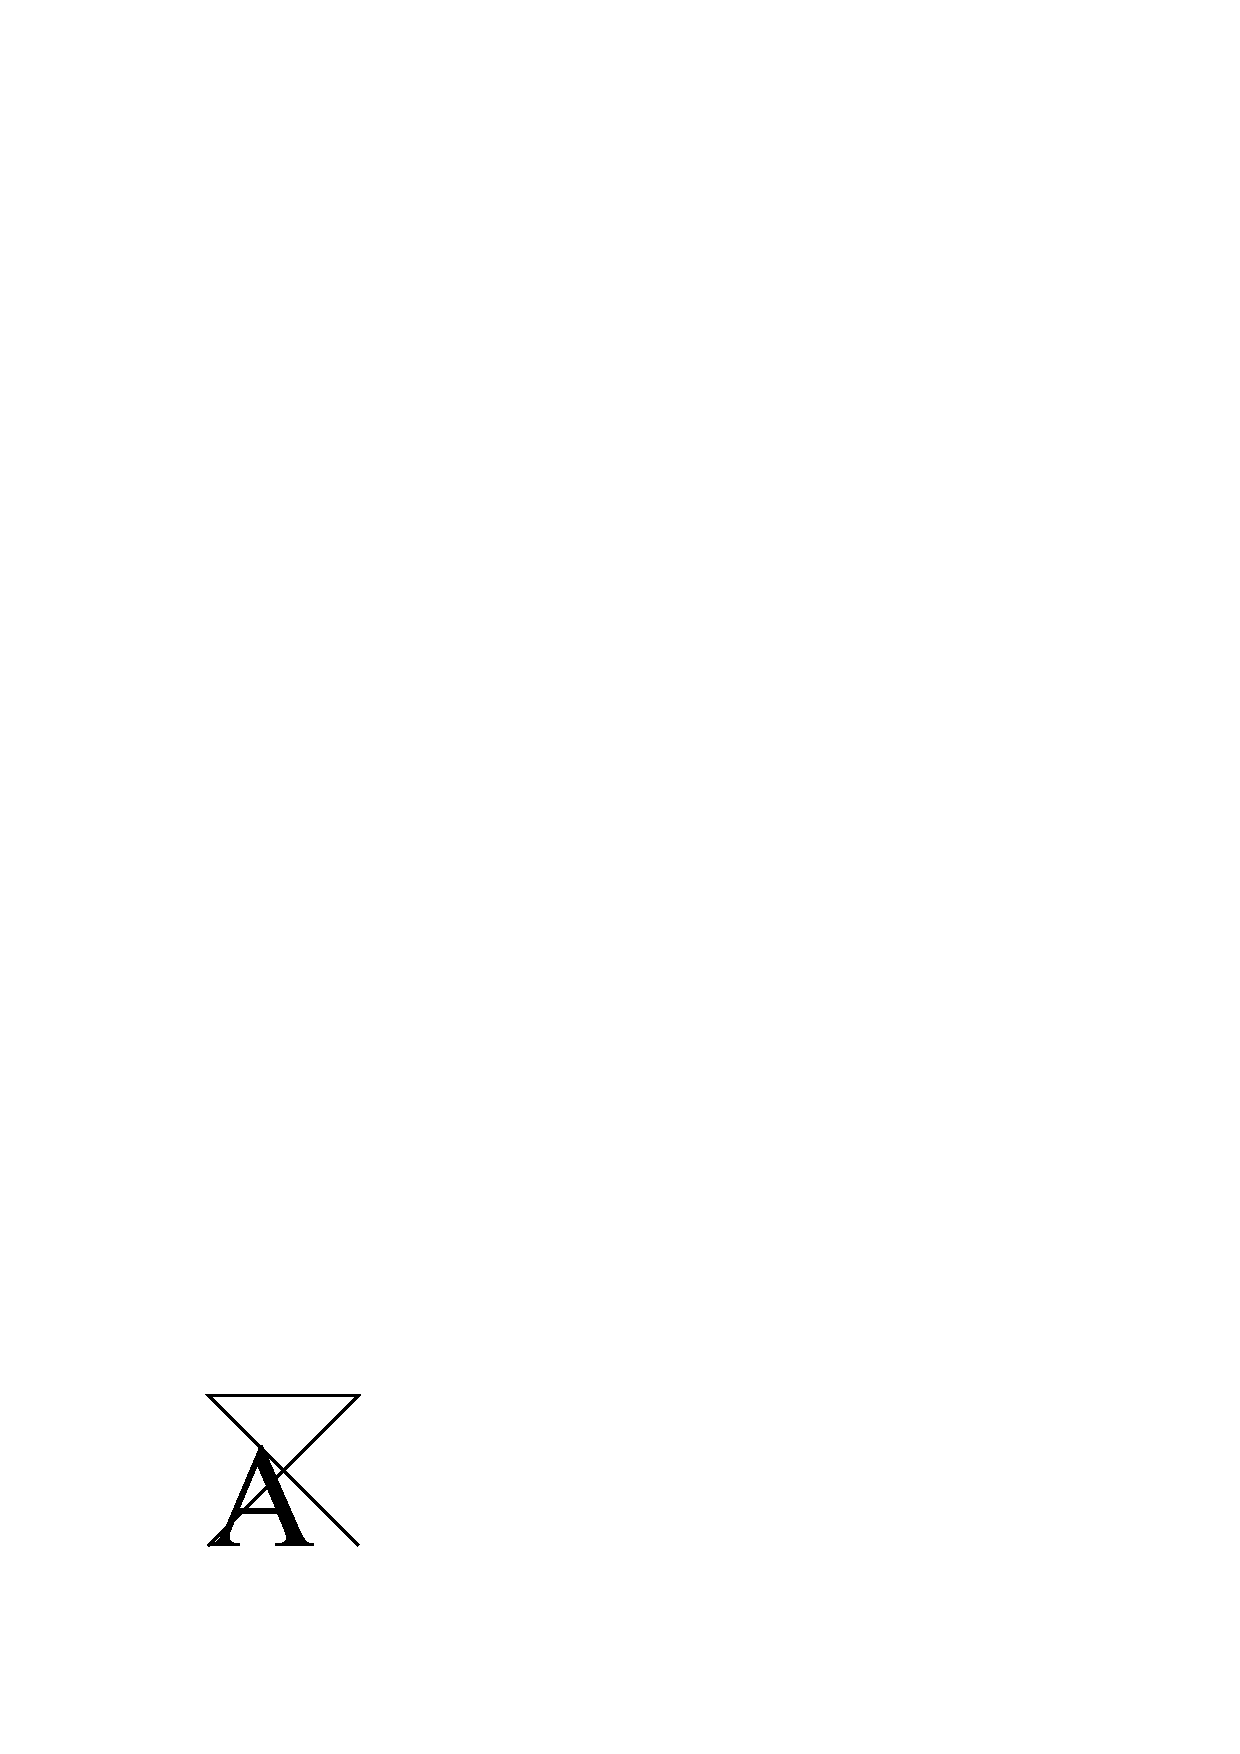
\includegraphics{a} ist ein Bild.
\exb
\begin{verbatim}
Hier 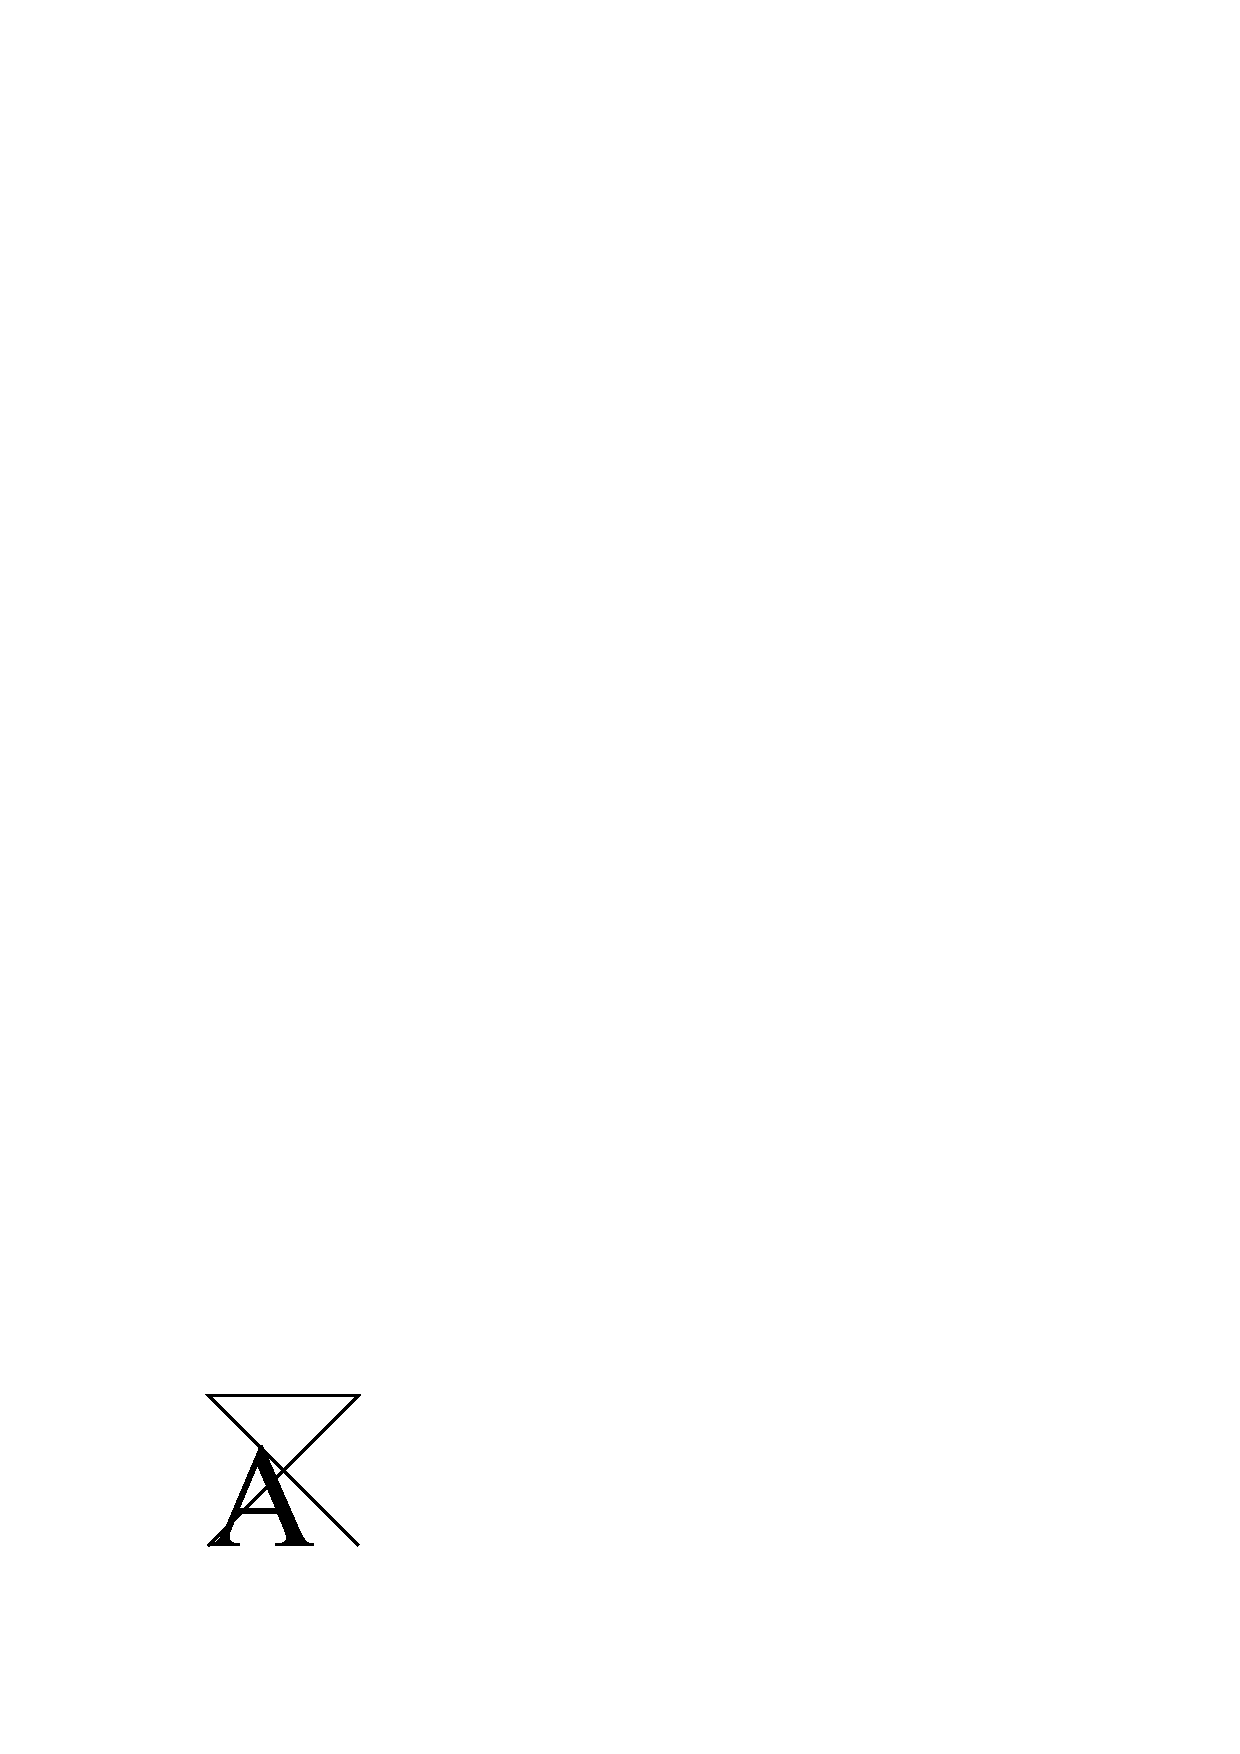
\includegraphics{a} ist
ein Bild
\end{verbatim}
\exc
Wird das Paket \texttt{graphicx} mit der Option \texttt{[draft]} geladen,
dann erscheint anstelle des Bildes nur ein Rahmen entsprechend
der tats"achlichen Bildgr"o"se mit dem Namen des Grafikfiles, 
was die Bearbeitung beschleunigt und f"ur Probeausdrucke n"utzlich ist.

Weitere Informationen zum Enbinden von Bildern finden Sie in der 
Online-Dokumentation \cite{grfguide}, im \textit{Graphics Companion}
\cite{grfcomp} und in K.~Reckdahls empfehlenswertem  Tutorium \cite{epslatex}.



\section{Seitenaufbau}

\subsection{Kopf- und Fu"szeilen} 
Der Inhalt von Kopf- und  Fu"szeilen kann mit dem Befehl
\begin{verse}
\verb|\pagestyle{|\textit{style}\verb|}|
\end{verse}
festgelegt werden:
 
Mit \verb|\pagestyle{plain}| steht
die Seitennummer zentriert in der Fu"szeile; 
das ist die Voreinstellung und braucht normalerweise nicht explizit 
angegeben zu werden.
Mit dem Stil \texttt{headings} stehen Kapitel-"Uberschrift und
Seitennummer in der Kopfzeile.
Mit \texttt{empty} sind Kopf- und Fu"szeile leer.  Der Befehl
\begin{verse}
\verb|\thispagestyle{|\textit{style}\verb|}|
\end{verse}
gilt entsprechend nur f"ur die aktuelle Seite.  Einige Befehle, wie etwa
\verb|\chapter|, "andern den Stil der aktuellen Seite.  Diese "Anderungen 
kann man durch einen nachfolgenden \verb|\thispagestyle|-Befehl aufheben.

\begin{sloppypar}%% `sloppypar'-Umgebung wegen vieler Befehle
\hbadness=4600\relax %% `underfull hbox'-Fehlermeldung aus
Im \manual\ ist angegeben, wie man das Aussehen der Kopf- und Fu"szeilen
au"serdem mit dem Seitenstil 
\verb|myheadings| und den Befehlen
\verb|\markboth|,
\verb|\markright| und
\verb|\pagenumbering|
beeinflussen kann.
\end{sloppypar}

\subsection{Gleitobjekte} \label{floats}
Gro"se Bilder und lange Tabellen lassen sich nicht immer genau 
dort unterbringen, wo sie inhaltlich hingeh"oren, weil sie nicht mehr 
vollst"andig auf die aktuelle Seite passen, aber auch nicht durch einen 
Seitenwechsel zerrissen werden sollen.  Um  solche Strukturen automatisch
an eine geeignete Stelle "`gleiten"' zu lassen, kennt \LaTeX{} die beiden 
Umgebungen \texttt{figure} und \texttt{table}.  

\subsubsection{Abbildungen (figure)}
Diese Umgebung ist f"ur die Behandlung von Abbildungen gedacht.
Tats"achlich spielt es aber keine Rolle, \emph{wie} diese erzeugt wurden:
Alles, was zwischen
\verb|\begin{figure}| und \verb|\end{figure}|
steht, wird automatisch an eine Stelle
gesetzt, wo es komplett hinpa"st, ohne durch einen Seitenwechsel
zerrissen zu werden.  

Mit \verb|\caption{...}| setzt man die Bezeichnung der Abbildung.
Dabei ist nur der Text anzugeben, das Wort "`Abbildung"' und die
fortlaufende Nummer werden von \LaTeX\ hinzu"-ge"-f"ugt.
Bei Abbildungen ist es allgemein "ublich, die Bezeichnung
\emph{unter} das Bild zu setzen.
Mit \verb|\label| und \verb|\ref| kann man die Nummer der
Abbildung im Text ansprechen, mit \verb|\pageref| ihre Seitenzahl.
Der Befehl \verb:\label: mu"s dabei \emph{nach} dem \verb:\caption:-Befehl
stehen, sonst stimmt die Numerierung nicht!

Im folgenden Beispiel wird einfach mit dem Befehl \verb|\vspace|
(siehe Abschnitt \ref{vabstaende})
leerer Raum f"ur ein sp"ater einzusetzendes Bild gelassen:
\exa
Abbildung~\ref{weiss} auf S.~\pageref{weiss} zeigt ein
Beispiel aus der Minimal art.
\exb
\begin{verbatim}
Abbildung~\ref{weiss} auf
S.~\pageref{weiss} zeigt
ein Beispiel aus der 
Minimal art.
\begin{figure}[tb]
\vspace{6cm}
\caption{Landschaft im
Nebel} \label{weiss}
\end{figure}
\end{verbatim}
\exc
\begin{figure}[tb]
\vspace{6cm}
\caption{Landschaft im
Nebel} \label{weiss}
\end{figure}

\LaTeX\ kann eine Abbildung nach verschiedenen Kriterien plazieren:
\texttt{h} "`here"' (hier),
\texttt{t} "`top"' (oben auf der Seite), \texttt{b} "`bottom"' (unten
auf der Seite) oder \texttt{p} "`page"' (eigene Seite f"ur
Abbildungen).

Die Parameter in den eckigen Klammern, die wahlweise angegeben
werden k"onnen, dienen dazu, die Plazierung der Abbildung auf die
angegebenen Orte \emph{ein"-zu"-schr"anken}.  Durch Angabe von
z.\,B.\ \texttt{tb}
wird \LaTeX{} angewiesen, nur eine Plazierung oben oder unten auf der
Seite zu versuchen, je nachdem,
wo \emph{zuerst} eine passende Stelle gefunden wird.
Werden keine Parameter (und keine eckigen
Klammern!) angegeben, ist die Voreinstellung \texttt{tbp},
also ohne~\texttt{h}.

Eine Plazierungsbeschr"ankung \emph{nur} auf \texttt{[h]} ist unsinnig;
sie w"urde das "`Gleiten"' ja gerade verhindern.
Wenn der Platz "`hier"' nicht ausreicht, 
verschiebt \LaTeX{} dann die Abbildung mindestens 
bis zum Anfang der n"achsten Seite, so als h"atte man \texttt{[ht]} angegeben.

Eine Abbildung, die nicht plaziert werden konnte, wird von
\LaTeX\ immer weiter nach hinten verschoben (und schiebt alle
weiteren Abbildungen vor sich her!), bis ein neues Kapitel
beginnt, das Dokument zu Ende ist, oder der Befehl
\verb|\clearpage| eingegeben wird.  


Es gibt noch einen weiteren Plazierungsparameter, 
\texttt{!}\ (bang), der \LaTeX{} anweist, 
gewisse eingebaute Beschr"ankungen zu ignorieren, 
z.\,B., da"s bei der Plazierung gem"a"s \texttt{h}, \texttt{t} oder \texttt{b}
ein Mindestanteil der Seite f"ur normalen Text "ubrig bleiben mu"s.
"`Bang"' mu"s immer zusammen mit mindestens einem der vier
anderen Parameter benutzt werden.  
 


\subsubsection{Tabellen (table)}

\begin{sloppypar}
\hbadness=3000\relax %% `underfull hbox'-Fehlermeldung aus

Damit Tabellen nicht auf einen Seitenwechsel fallen,
k"onnen sie, analog zu Abbildungen, zwischen
\verb|\begin{table}| und \verb|\end{table}| gesetzt werden.
Die Befehle
\verb|\caption|, \verb|\label|, \verb|\ref| und \verb|\pageref|
wirken entsprechend.
Hier sind beide m"og"-lichen Konventionen verbreitet: Die
Bezeichnung wird entweder immer \emph{"uber} oder immer
\emph{unter} die Tabelle gesetzt.
\end{sloppypar}

Auch hier gilt, da"s in der \texttt{table}-Umgebung  beliebiger
Text stehen darf; die Tabelle mu"s nicht zwangsl"aufig durch die
\texttt{tabular}-Umgebung erzeugt worden sein.
Der Unterschied zu \texttt{figure} besteht nur darin, 
da"s die Bezeichnung mit dem Wort "`Tabelle"' versehen wird,
und da"s die Tabellen unabh"angig von den Abbildungen numeriert werden.

\endinput

\clearpage

% master: l2kurz.tex
% l2k5.tex - 5.Teil der LaTeX2e-Kurzbeschreibung v2.3
% 2001-04-10 (WaS)

\section{Schriften}
Normalerweise w"ahlt \LaTeX\ die Gr"o"se und den Stil der Schrift
aufgrund der Befehle aus, die die logische Struktur des Textes angeben:
"Uber"-schriften, Fu"snoten, Hervorhebungen usw.
Im folgenden werden Befehle und Makropakete beschrieben, mit denen
die Schrift auch explizit beeinflu"st werden kann.
Ausf"uhrlichere Erl"auterungen zum Umgang mit Schriften in \LaTeX{}
findet man im \textit{\LaTeX-Begleiter} \cite{wonne}
und in der Online-Dokumentation \cite{fntguide}.



\subsection{Schriftgr"o"sen}
 
Die in der Tabelle~\ref{sizes} an"-ge"-f"uhrten Befehlen 
wechseln die Schriftgr"o"se.
Sie spezifizieren die Gr"o"se relativ
zu der von \verb:\documentclass: festgelegten Grundschrift.
Ihr Wirkung reicht bis zum Ende der aktuellen Gruppe oder Umgebung.


\begin{table}[hb]
\caption{Schriftgr"o"sen} \label{sizes}
\oben{10cm}
\begin{tabbing}
\texttt{xfootnotesizexx}\= und dann der Text \kill
\verb|\tiny|         \> \tiny        winzig kleine Schrift \\
\verb|\scriptsize|   \> \scriptsize  sehr kleine Schrift (wie Indizes)\\
\verb|\footnotesize| \> \footnotesize     kleine Schrift (wie Fu"snoten)\\
\verb|\small|        \> \small            kleine Schrift \\
\verb|\normalsize|   \> \normalsize  normale Schrift \\
\verb|\large|        \> \large       gro"se Schrift \\
\verb|\Large|        \> \Large       gr"o"sere Schrift \\
\verb|\LARGE|        \> \LARGE       sehr gro"se Schrift \\[3pt]
\verb|\huge|         \> \huge        riesig gro"s \\[3pt]
\verb|\Huge|         \> \Huge        gigantisch
\end{tabbing}
\unten
\end{table}
 
Die Gr"o"sen-Befehle ver"andern auch die Zeilen"-ab"-st"ande auf
die jeweils passenden Werte -- aber nur, wenn die
Leerzeile, die den Absatz be\-en\-det, innerhalb des
G"ultigkeitsbereichs des Gr"o"sen-Befehls liegt:
\exa
{\Large zu enger\\
Abstand}\par
\exb
\begin{verbatim}
{\Large zu enger \\
Abstand}\par
\end{verbatim}
\exc
\exa
{\Large richtiger\\
Abstand\par}
\exb
\begin{verbatim}
{\Large richtiger\\
Abstand\par}
\end{verbatim}
\exc
F"ur korrekte
Zeilen"-ab"-st"ande darf die
schlie"-"sende geschwungene Klammer also nicht zu fr"uh kommen,
sondern erst nach einem Absatzende, das "ubrigens nicht nur als
Leerzeile, sondern auch als Befehl \verb|\par|  eingegeben werden 
kann.


\subsection{Schriftstil}
Der Schriftstil wird in \LaTeX{} durch 3~Merkmale definiert:
\begin{description}
\item[Familie] Standardm"a"sig stehen 3~Familien zur Wahl:
  "`roman"' (Antiqua), "`sans serif"' (Serifenlose) und "`typewriter"'
  (Schreibmaschinenschrift).
\item[Serie] Die Serie gibt St"arke und Laufweite der
  Schrift an: "`medium"' (normale Schrift), "`boldface extended"'
  (fett und breiter).
\item[Form] Die Form der Buchstaben: "`upright"'
  (aufrecht), "`slanted"' (geneigt), "`italic"' (kursiv),
  "`caps and small caps"' (Kapit"alchen).
\end{description}
Tabelle~\ref{fonts} zeigt die Befehle, mit denen diese Attribute 
explizit beeinflu"st werden k"onnen.  
Die Befehle der Form \verb|\text...| setzen nur ihr Argument im 
gew"unschten  Stil.  Zu jedem dieser Befehle ist ein Gegenst"uck angegeben, 
das von seinem Auf\/treten an bis zum Ende der laufenden Gruppe oder Umgebung 
wirkt.

Zu beachten ist, da"s W"orter in Schreibmaschinenschrift nicht automatisch
getrennt werden.\par

\begin{table}[hbp]
\caption{Schriftstile} \label{fonts}
\oben{10cm}
\begin{tabbing}\small
\verb|\textnormal|\{\textit{text}\}\qquad\=\verb|\normalfont|\qquad\=\kill
\verb|\textrm|\{\textit{text}\}         \>\verb|\rmfamily|       \>\textrm{Antiqua}\\
\verb|\textsf|\{\textit{text}\}         \>\verb|\sffamily|       \>\textsf{Serifenlose}\\
\verb|\texttt|\{\textit{text}\}         \>\verb|\ttfamily|       \>\texttt{Maschinenschrift}\\[1ex]
\verb|\textmd|\{\textit{text}\}         \>\verb|\mdseries|       \>\textmd{normal}\\
\verb|\textbf|\{\textit{text}\}         \>\verb|\bfseries|       \>\textbf{fett, breiter laufend}\\[1ex]
\verb|\textup|\{\textit{text}\}         \>\verb|\upshape|        \>\textup{aufrecht}\\
\verb|\textsl|\{\textit{text}\}         \>\verb|\slshape|        \>\textsl{geneigt}\\
\verb|\textit|\{\textit{text}\}         \>\verb|\itshape|        \>\textit{kursiv}\\
\verb|\textsc|\{\textit{text}\}         \>\verb|\scshape|        \>\textsc{Kapit"alchen}\\[1ex]
\verb|\textnormal|\{\textit{text}\}     \>\verb|\normalfont|     \>\textnormal{Die Grundschrift des Dokuments}
\end{tabbing}
\unten
\end{table}

Die Befehle f"ur Familie, Serie und Form k"onnen untereinander und mit den
Gr"o"sen-Befehlen kombiniert werden;  allerdings mu"s nicht jede
m"ogliche Kombination tats"achlich als reale Schrift (Font)
zur Verf"ugung stehen.
\exa
{\small Die kleinen
\textbf{fetten} R"omer
beherrschten }{\large das
ganze gro"se \textit{Italien}.}
\\[6ex]
{\Large\sffamily\slshape plakativ}
\exb
\begin{verbatim}
{\small Die kleinen
\textbf{fetten} R"omer
beherrschten }{\large das
ganze gro"se \textit{Italien}.}
{\Large\sffamily\slshape plakativ}
\end{verbatim}
\exc

Je \emph{weniger} verschiedene Schriftarten man verwendet, desto
lesbarer und sch"oner wird das Schrift"-st"uck!


\subsection{Andere Schriftfamilien}
Mit den im vorigen Abschnitt eingef"uhrten Befehlen kann man nicht beeinflussen,
welche Schriftfamilien tats"achlich als Antiqua, Serifenlose und
Maschinenschrift benutzt werden.  \LaTeX{} verwendet als Voreinstellung
die sog.\ Computer-Modern-Schriftfamilien (CM), siehe Tabelle~\ref{families};
der Stil der mathematischen Zeichens"atze pa"st dabei zu CM~Roman.

Will man andere Schriften benutzen, dann ist der einfachste Weg 
das Laden eines Pakets, das eine oder mehrere dieser Schriftfamilien 
komplett ersetzt.
Tabelle~\ref{families} f"uhrt einige derartige Pakete auf%,
% die allerdings nicht in jeder \LaTeX-Installation verf"ugbar sein m"ussen
.

Die Dokumentation Ihres \TeX-Systems \cite{local} sollte dar"uber
informieren, welche Schriften verf"ugbar sind
und wie Sie weitere installieren und verwenden k"onnen.
Insbsondere sollte eine Anzahl von verbreiteten PostScript-Schriften
mit jedem aktuellen \LaTeX-System verwendbar sein \cite{postscript}.

\begin{table}[htb]
\caption[Pakete f"ur alternative Schriftfamilien]
{Pakete f"ur alternative Schriftfamilien (Eine leere
Tabellenspalte bedeutet, da"s das Paket die betreffende Schriftfamilie nicht 
ver"andert; * kennzeichnet die jeweils als Grundschrift eingestellte Familie.)}
\label{families}
{\footnotesize
\begin{center}
\medskip
\renewcommand{\arraystretch}{1.5}
\begin{tabular}{|l|p{2.cm}p{2.2cm}p{2.4cm}p{2.2cm}|}
\hline
Paket            & Antiqua    & Serifenlose   & Schreibmaschine  & math.\ Formeln\\\hline\hline
(keines)         & CM Roman * & CM Sans Serif & CM Typewriter    & $\approx$ CM Roman\\\hline
\texttt{ccfonts} & Concrete *
                 &
                 &
                 & $\approx$ Concrete\\\hline
\texttt{cmbright}&
                 & CM Bright *
                 & {\raggedright CM\ Typewriter\\ Light}
                 & $\approx$ CM Bright\\\hline
% \texttt{pandora} & {\raggedright Pandora\\ Roman *} 
%                  & {\raggedright Pandora \\ Sans Serif} 
%                  &
%                  & \\\hline
\texttt{mathptmx}& Times *
                 &
                 &
                 & $\approx$ Times\\\hline
\texttt{mathpazo}& Palatino *
                 &
                 &
                 & $\approx$ Palatino\\\hline
\texttt{helvet}  & 
                 & Helvetica
                 &
                 & \\\hline
\texttt{courier} &
                 &
                 & Courier 
                 & \\\hline
\end{tabular}
\end{center}
}
\end{table}


\subsection{Die "`europ"aischen"' Zeichens"atze}
\LaTeX{} verwendet standardm"a"sig  Schriften mit einem Umfang von
128~Zeichen.  Umlaute oder akzentuierte Buchstaben sind darin nicht
enthalten; sie werden jeweils aus dem Grundsymbol und dem Akzent
zusammengesetzt.  

Inzwischen stehen die meisten der mit \LaTeX\ verwendbaren Schriften
auch mit einem erweiterten "`europ"aischen"' Zeichenvorrat bereit.
Sie enthalten jetzt 256 Zeichen, welche fast
alle europ"aischen Sprachen abdecken, d.\,h., jedes be\-n"o\-tig\-te
Zeichen ist vorgefertigt in ihnen enthalten.
Das hat nicht nur eine
h"ohere typographische Qualit"at zur Folge; aufgrund der inneren Arbeitsweise
von \TeX{} entfallen damit auch die Einschr"ankungen im Zusammenhang mit
der Silbentrennung, die im Abschnitt~\ref{silb} erw"ahnt wurden:
W"orter mit Umlauten werden nun besser getrennt, und im Argument des
Befehls \verb|\hyphenation| d"urfen auch Umlaute und das scharfe~s stehen.

%% stimmt nur fuer EC
%Weiterhin sind die Unterschneidungen im Vergleich zu den amerikanischen
%\TeX-Originalschriften stark verbessert und nun auch auf h"aufige
%Buchstabenpaarungen in nicht-englischen Sprachen optimiert.

% <------- Formulierung ????
Die europ"aischen Schriften bestehen aus zwei Teilen: Der T1-Zeichensatz
enth"alt Buchstaben, ASCII-Zeichen sowie verschiedene Anf"uhrungszeichen
und Striche, 
w"ahrend ein erg"anzender TS1-Zeichensatz zu\-s"atz\-liche Textsymbole bereitstellt.
% <------- Formulierung ????

\LaTeX{} wird veranla"st, T1-Schriften zu verwenden,
indem man das Paket \texttt{fontenc} mit der Option \texttt{T1} l"adt:
\begin{quote}
  \verb|\usepackage[T1]{fontenc}|
\end{quote}
Das Paket \texttt{textcomp} erm"oglicht den Zugriff auf die Textsymbole:
\begin{quote}
  \verb|\usepackage{textcomp}|
\end{quote}
Welche zus"atzlichen Zeichen mit den T1-Schriften
bereitgestellt werden, ist in \cite{usrguide} zusammengefa"st;
Anhang~\ref{textsymbols} der vorliegenden Kurzbeschreibung
enth"alt eine Liste aller TS1-Textsymbole.  Einige der Textsymbole sind
auch ohne das Paket \texttt{textcomp} verf"ugbar, siehe Abschnitt~\ref{symbole},
dann aber nicht immer in einem zur laufenden Schrift passenden Stil.

Beachten Sie, da"s in Fonts, die nicht speziell f"ur die Verwendung 
mit \TeX\ entworfen wurden, 
nur ein Teil der TS1-Textsymbole enthalten ist.
Das betrifft vor allem die "`handels"ublichen"' PostScript-Schriften.

\endinput


\clearpage

% master: l2kurz.tex
% l2k6.tex - 6.Teil der LaTeX2e-Kurzbeschreibung v2.3
% 2003-04-10 (WaS)

\section{Spezialitäten}
 
Das komplette Menü der Spezialitäten, die von \LaTeX\ serviert
werden, ist im \manual\ und in der Online-Dokumentation beschrieben.
Hier soll nur auf einige besondere "`Schmankerln"' hingewiesen
werden.
 
\subsection{Abstände}

\subsubsection{Zeilenabstand}

Um in einem Schriftstück größere Zeilenabstände zu verwenden,
als es in der Dokumentklasse vorgesehen ist, gibt es in
\LaTeX\ den Befehl \verb:\linespread:, der im Vorspann stehen sollte
und dann auf das gesamte Dokument wirkt.  Das kann beispielsweise
dann notwendig werden, wenn eine Schrift benutzt wird, die eine größerer x-Höhe 
hat als die voreingestellte Computer-Modern.  Für die Schrift "`Palatino"' etwa
ist eine Vergrößerung des Zeilenabstandes um ca.\ 5\,\% angemessen:

\begin{quote}
\verb|\usepackage{mathpazo}|\\
\verb|\linespread{1.05}|
\end{quote}

 
 
 
\subsubsection{Spezielle horizontale Abstände}\label{abst:horiz}
 
Die Abstände zwischen Wörtern und Sätzen werden von \LaTeX\ 
automatisch gesetzt.
Sonstigen horizontalen Abstand kann man mit dem Befehl
\begin{verse}
\verb|\hspace{|\textit{länge}\verb|}|
\end{verse}
einfügen.
Wenn der Abstand auch am Beginn oder Ende einer Zeile
erhalten bleiben soll, muss \verb|\hspace*| statt \verb|\hspace|
geschrieben werden.
Die Längenangabe besteht im einfachsten Fall aus einer Zahl
und einer Einheit.  Die wichtigsten Einheiten sind in
Tabelle~\ref{units} angeführt.
\begin{table}[b]
\caption{Einheiten für Längenangaben} \label{units}
\oben{11cm}
\begin{tabbing}
\texttt{mm}\qquad \= Millimeter                               \\
\texttt{cm} \> Zentimeter = 10\,mm                            \\
\texttt{in} \> inch \(= 25.4\,\mathrm{mm} \)                  \\
\texttt{pt} \> point \( =(1/72.27)\,\mathrm{in}
                        \approx 0.351\,\mathrm{mm}\)          \\
\texttt{bp} \> big point \( =(1/72)\,\mathrm{in}
                            \approx 0.353\,\mathrm{mm} \)      \\
%\texttt{dd} \> Didot-Punkt \( = (1238/1157)\,\mathrm{pt}
%                              \approx 0.376\,\mathrm{mm} \)   \\
% --- wegen unklarer Definition (0.375 ider 0.376mm) besser nicht benutzen!
\texttt{em} \> Geviert (doppelte Breite einer Ziffer der aktuellen Schrift)\\
\texttt{ex} \> Höhe des Buchstabens x der aktuellen Schrift
\end{tabbing}                    
\unten
\end{table}
Die Befehle in Tabelle~\ref{hspace} sind Abkürzungen zum Einfügen
besonderer horizontaler Abstände.
\begin{table}[t]
\caption{Befehle für horizontale Abstände} \label{hspace}
\oben{13cm}
\begin{tabbing}
\texttt{xenspace}\qquad \= \kill
\verb|\,|       \> ein sehr kleiner Abstand (siehe auch Abschnitt~\ref{abstaende})\\
\verb|\enspace| \> so breit wie eine Ziffer \\
\verb|\quad|    \> so breit, wie ein Buchstabe hoch ist
                   ("`weißes Quadrat"') \\
\verb|\qquad|   \> doppelt so breit wie ein \verb|\quad| \\
\verb|\hfill|   \> ein Abstand, der sich von 0 bis \(\infty\)
                   ausdehnen kann.
\end{tabbing}
\unten
\end{table}
Der Befehl \verb|\hfill| kann dazu dienen, einen vorgegebenen
Platz auszufüllen.
\exa
\raggedright
Schafft mir\hspace{1.5cm}Raum! \\
\(\triangleleft\)\hfill \(\triangleright\)\\
\exb
\begin{verbatim}
Schafft mir\hspace{1.5cm}Raum! \\
\(\triangleleft\)\hfill 
\(\triangleright\)
\end{verbatim}
\exc


\subsubsection{Spezielle vertikale Abstände} \label{vabstaende}
 
Die Abstände zwischen Absätzen, Kapiteln usw.\ werden von
\LaTeX\ automatisch bestimmt.
In Spezialfällen kann man zusätzlichen Abstand
\emph{zwischen zwei Absätzen} mit dem Befehl
\begin{verse}
\verb|\vspace{|\textit{länge}\verb|}|
\end{verse}
bewirken.
Dieser Befehl sollte immer zwischen zwei Leerzeilen angegeben
werden.
Wenn der Abstand auch am Beginn oder Ende einer Seite erhalten
bleiben soll, muss \verb|\vspace*| statt \verb|\vspace|
geschrieben werden.
Die Befehle in Tabelle~\ref{vspace} sind Abkürzungen für
bestimmte vertikale Abstände.
\begin{table}[t]
\caption{Befehle für vertikale Abstände} \label{vspace}
\oben{13cm}
\begin{tabbing}
\texttt{xsmallskip}\qquad \= \kill
\verb|\smallskip| \> etwa \(\nfrac{1}{4}\) Zeile \\
\verb|\medskip|   \> etwa \(\nfrac{1}{2}\) Zeile \\
\verb|\bigskip|   \> etwa 1 Zeile \\
\verb|\vfill|     \> ein Abstand, der sich von 0 bis \(\infty\)
                     ausdehnen kann
\end{tabbing}
\unten
\end{table}
Der Befehl \verb|\vfill| in Verbindung mit \verb|\newpage|
kann dazu dienen, Text an den unteren Rand einer Seite zu setzen
oder vertikal zu zentrieren.  Beispielsweise enthält der Quelltext
für die zweite Seite der vorliegenden Beschreibung:
\begin{quote}
\begin{verbatim}
\vfill

Dieses Dokument wurde mit \LaTeX{} gesetzt.
...
\newpage
\end{verbatim}
\end{quote}
 
Zusätzlichen Abstand zwischen zwei Zeilen \emph{innerhalb}
eines Absatzes oder einer Tabelle erreicht man mit dem Befehl
\verb|\\[|\textit{länge}\verb|]|.
\exa
Albano Cesara \\
Lindenallee 10 \\[1.5ex]
95632 Pestitz
\exb
\begin{verbatim}
Albano Cesara \\
Lindenallee 10 \\[1.5ex]
95632 Pestitz
\end{verbatim}
\exc

\smallskip
 
 
\subsection{Briefe}\label{briefe}
 
Mit der Dokumentklasse \texttt{letter} kann man zwischen
\verb|\begin{document}| und \verb|\end{document}| einen oder
mehrere Briefe schreiben. 
Abbildung~\ref{brief} enthält ein Beispiel für einen Brief.

\begin{figure}[ht] %\small
\oben{11cm}
\begin{alltt}
\verb+\documentclass[12pt,a4paper]{letter}+
\verb+\usepackage[latin1]{inputenc}+
\verb+\usepackage{german}+
\verb+\address{EDV-Zentrum der TU Wien \\+
\verb+  Abt. Digitalrechenanlage \\+
\verb+  +Wiedner Hauptstra\ss{}e 8--10 \verb+\\+
\verb+  A-1040 Wien}+
\verb+\signature{Dr. Hubert Partl}+
\verb+\begin{document}+
\verb+\begin{letter}{Frau Mag. Elisabeth Schlegl \\+
\verb+  +EDV-Zentrum der Karl-Franzens-Universit\"at \verb+\\+
\verb+  Attemsgasse 25/II \\+
\verb+  \textbf{A-8010 Graz}}+
\verb+\opening{Liebe Frau Schlegl,}+
herzlichen Dank f\"ur die Zusendung \dots

\dots in etwa 2--3~Wochen fertig zu sein.
\verb+\closing{+Mit freundlichen Gr\"u\ss{}en\verb+}+
\verb+\end{letter}+
\verb+\end{document}+
\end{alltt}
\unten
\caption{Brief von H.\,P. an E.\,S.} \label{brief}
\end{figure}

Mit dem Befehl \verb|\address| definiert man die Adresse des Absenders.
\verb|\begin{letter}{...}| beginnt einen Brief an den im
Parameter angegebenen Empfänger.
\verb|\opening{...}| schreibt die Anrede 
und \verb|\closing{...}| den abschließenden Gruß, 
an den automatisch die eingangs mit
\verb|\signature| vereinbarte Unterschrift angefügt wird.
\verb|\end{letter}| beendet den jeweiligen Brief.

Das von der Dokumentklasse \texttt{letter} bewirkte Layout der Briefe 
orientiert sich an amerikanischen Gepflogenheiten.
Mit vielen \LaTeX-Systemen ist die Klasse 
\texttt{dinbrief} verfügbar; sie setzt die Briefe in einer
Anordnung gemäß DIN~676, 
die für die Verwendung von A4-Bogen in Fensterkuverts geeignet ist.
Der \local{} sollte Auskunft über diese oder andere Alternativen zu
\texttt{letter} geben.

\subsection{Literaturangaben}

Mit der \texttt{thebibliography}-Umgebung kann man ein
Literaturverzeichnis erzeugen.
Darin beginnt jede Literaturangabe mit \verb|\bibitem|.
Als Parameter wird ein Name vereinbart, unter dem die
Literaturstelle im Text zitiert werden kann, und
dann folgt der Text der Literaturangabe.
Die Nummerierung erfolgt automatisch.
Der Parameter bei \verb|\begin{thebibliography}| gibt die
maximale Breite dieser Nummernangabe an, also z.\,B.\ 
\verb|{99}| für maximal zweistellige Nummern.

Im Text zitiert man die Literaturstelle dann mit dem Befehl \verb|\cite|
und dem vereinbarten Namen als Argument.
\exa
Partl~\cite{pa} hat
vorgeschlagen, dass \dots
 
\begin{thebibliography}{99}
\bibitem{pa}
H.~Partl: \textit{German \TeX,}
TUG\-boat Vol.~9, No.~1 (1988)
\end{thebibliography}
\exb
\begin{verbatim}
Partl~\cite{pa} hat
vorgeschlagen ...
 
\begin{thebibliography}{99}
\bibitem{pa}
H.~Partl: \textit{German \TeX,}
TUGboat Vol.~9, No.~1 (1988)
\end{thebibliography}
\end{verbatim}
\exc

 
\subsection{Zerbrechliche Befehle}
 
Manche \LaTeX-Befehle "`verfrachten"' ihre Argumente an eine andere
Stelle im Text; beispielsweise kann das Argument von \verb|\section|
auch im Inhaltsverzeichnis und möglicherweise in der Kopfzeile auftauchen.  

Bestimmte Befehle "`überstehen"' diesen Transport nicht, wenn sie
ohne besondere Maßnahmen in einem solchen "`beweglichen Argument"'
auftreten.
Derartige Befehle heißen "`zerbrechlich"'.  Damit sie dennoch innnerhalb
von beweglichen Argumenten benutzt werden dürfen, 
muss man ihnen einfach den Befehl \verb|\protect| voranstellen.

Zerbrechlich sind insbesondere alle Befehle, die ein optionales Argument
kennen, also auch \verb|\\| (sic!),
außerdem die Befehle \verb|\(|, \verb|\)| und \verb|\footnote|.

Bewegliche Argumente haben, neben den Gliederungsbefehlen,
auch der Befehl \verb|\caption| und die Umgebung \texttt{letter}.


\endinput

\clearpage

% master: l2kurz.tex
% L2KA.TEX - Anhang der LaTeX-Kurzbeschreibung v2.2
% 2001-06-08 (WaS)

\appendix
%\settocdepth{1}

\enlargethispage*{2.5\baselineskip}

\section{Mit dem Paket \texttt{textcomp} verfügbare Symbole}
\label{textsymbols}
{\small
\begin{tabbing}
\quad\quad\=\texttt{Mtextquotestraightdblbase}\hspace{1cm}\=\quad\quad\=\kill
\textquotestraightbase \> \verb+\textquotestraightbase+\textsuperscript{*}  \> \textquotestraightdblbase \> \verb+\textquotestraightdblbase+\textsuperscript{*} \\
\texttwelveudash \> \verb+\texttwelveudash+\textsuperscript{*}  \> \textthreequartersemdash \> \verb+\textthreequartersemdash+\textsuperscript{*} \\
\textleftarrow \> \verb+\textleftarrow+ \> \textrightarrow \> \verb+\textrightarrow+\\
\textblank \> \verb+\textblank+ \> \textdollar \> \verb+\$+\textsuperscript{*} \\
\textquotesingle \> \verb+\textquotesingle+\textsuperscript{*}  \> \textasteriskcentered \> \verb+\textasteriskcentered+\textsuperscript{*} \\
\textdblhyphen \> \verb+\textdblhyphen+ \> \textfractionsolidus \> \verb+\textfractionsolidus+\textsuperscript{*} \\
\textlangle \> \verb+\textlangle+ \> \textminus \> \verb+\textminus+\textsuperscript{*} \\
\textrangle \> \verb+\textrangle+ \> \textmho \> \verb+\textmho+\\
\textbigcircle \> \verb+\textbigcircle+ \> \textohm \> \verb+\textohm+\\
\textlbrackdbl \> \verb+\textlbrackdbl+ \> \textrbrackdbl \> \verb+\textrbrackdbl+\\
\textuparrow \> \verb+\textuparrow+ \> \textdownarrow \> \verb+\textdownarrow+\\
\textasciigrave \> \verb+\textasciigrave+\textsuperscript{*}  \> \textborn \> \verb+\textborn+\\
\textdivorced \> \verb+\textdivorced+ \> \textdied \> \verb+\textdied+\\
\textleaf \> \verb+\textleaf+ \> \textmarried \> \verb+\textmarried+\\
\textmusicalnote \> \verb+\textmusicalnote+ \> \texttildelow \> \verb+\texttildelow+\textsuperscript{*} \\
\textdblhyphenchar \> \verb+\textdblhyphenchar+ \> \textasciibreve \> \verb+\textasciibreve+\textsuperscript{*} \\
\textasciicaron \> \verb+\textasciicaron+\textsuperscript{*}  \> \textacutedbl \> \verb+\textacutedbl+\textsuperscript{*} \\
\textgravedbl \> \verb+\textgravedbl+\textsuperscript{*}  \> \textdagger \> \verb+\dag+\textsuperscript{*} \\
\textdaggerdbl \> \verb+\ddag+\textsuperscript{*} \> \textbardbl \> \verb+\textbardbl+\textsuperscript{*} \\
\textperthousand \> \verb+\textperthousand+\textsuperscript{*} \> \textbullet \> \verb+\textbullet+\textsuperscript{*} \\
\textcelsius \> \verb+\textcelsius+\textsuperscript{*}  \> \textdollaroldstyle \> \verb+\textdollaroldstyle+\\
\textcentoldstyle \> \verb+\textcentoldstyle+ \> \textflorin \> \verb+\textflorin+\textsuperscript{*} \\
\textcolonmonetary \> \verb+\textcolonmonetary+ \> \textwon \> \verb+\textwon+\\
\textnaira \> \verb+\textnaira+ \> \textguarani \> \verb+\textguarani+\\
\textpeso \> \verb+\textpeso+ \> \textlira \> \verb+\textlira+\\
\textrecipe \> \verb+\textrecipe+ \> \textinterrobang \> \verb+\textinterrobang+\\
\textinterrobangdown \> \verb+\textinterrobangdown+ \> \textdong \> \verb+\textdong+\\
\texttrademark \> \verb+\texttrademark+\textsuperscript{*} \> \textpertenthousand \> \verb+\textpertenthousand+\\
\textpilcrow \> \verb+\textpilcrow+ \> \textbaht \> \verb+\textbaht+\\
\textnumero \> \verb+\textnumero+ \> \textdiscount \> \verb+\textdiscount+\\
\textestimated \> \verb+\textestimated+ \> \textopenbullet \> \verb+\textopenbullet+\\
\textservicemark \> \verb+\textservicemark+ \> \textlquill \> \verb+\textlquill+\\
\textrquill \> \verb+\textrquill+ \> \textcent \> \verb+\textcent+\textsuperscript{*} \\
\textsterling \> \verb+\pounds+\textsuperscript{*}  \> \textcurrency \> \verb+\textcurrency+\textsuperscript{*} \\
\textyen \> \verb+\textyen+\textsuperscript{*} \> \textbrokenbar \> \verb+\textbrokenbar+\textsuperscript{*} \\
\textsection \> \verb+\S+\textsuperscript{*}  \> \textasciidieresis \> \verb+\textasciidieresis+\textsuperscript{*} \\
\textcopyright \> \verb+\copyright+\textsuperscript{*} \> \textordfeminine \> \verb+\textordfeminine+\textsuperscript{*} \\
\textcopyleft \> \verb+\textcopyleft+ \> \textlnot \> \verb+\textlnot+\textsuperscript{*} \\
\textcircledP \> \verb+\textcircledP+ \> \textregistered \> \verb+\textregistered+\textsuperscript{*} \\
\textasciimacron \> \verb+\textasciimacron+\textsuperscript{*}  \> \textdegree \> \verb+\textdegree+\textsuperscript{*} \\
\textpm \> \verb+\textpm+\textsuperscript{*} \> \texttwosuperior \> \verb+\texttwosuperior+\\
\textthreesuperior \> \verb+\textthreesuperior+ \> \textasciiacute \> \verb+\textasciiacute+\textsuperscript{*} \\
\textmu \> \verb+\textmu+\textsuperscript{*} \> \textparagraph \> \verb+\P+\textsuperscript{*} \\
\textperiodcentered \> \verb+\textperiodcentered+\textsuperscript{*} \> \textreferencemark \> \verb+\textreferencemark+\\
\textonesuperior \> \verb+\textonesuperior+ \> \textordmasculine \> \verb+\textordmasculine+\textsuperscript{*} \\
\textsurd \> \verb+\textsurd+ \> \textonequarter \> \verb+\textonequarter+\\
\textonehalf \> \verb+\textonehalf+ \> \textthreequarters \> \verb+\textthreequarters+\\
\textsf{\texteuro} \> \verb+\textsf{\texteuro}+ \> \texttimes \> \verb+\texttimes+\textsuperscript{*} \\
\textdiv \> \verb+\textdiv+\textsuperscript{*} \\
\end{tabbing}
}

{\footnotesize\noindent 
Schriften, die nicht speziell für die Verwendung mit
\TeX{} entworfen wurden, enthalten normalerweise nur die mit * markierten Zeichen.
\par}


\endinput

\clearpage

\begin{thebibliography}{99} \hbadness10000 % wg. URLs ;-)
 
\bibitem{manual}
L.~Lamport: \textit{Das \LaTeX-Handbuch.}
Addison-Wesley Deutschland (1995)%, ISBN~3-89319-826-1
. Deutsche "Uber"-setzung von~\cite{manual-eng}.

\bibitem{manual-eng}
L.~Lamport: \textit{\LaTeX, A Document Preparation System.}
Ad\-di\-son-Wesley, 2.~Aufl. (1994)%, ISBN~0-201-52983-1
.
 
\bibitem{wonne}
M.~Goossens, F.~Mittelbach und A.~Samarin:
\textit{Der \LaTeX-Begleiter.}
Ad\-di\-son Wesley Longman, 2.~korr.\ Nachdruck (1996)%, ISBN~3-89319-646-3
.  Deutsche "Uber"-setzung von~\cite{wonne-eng}.

\bibitem{wonne-eng}
M.~Goossens, F.~Mittelbach und A.~Samarin:
\textit{The \LaTeX\ Companion.}
Ad\-di\-son-Wesley (1994)%, ISBN~0-201-54199-8
.  

\bibitem{ch8}
M.~Goossens, F.~Mittelbach und A.~Samarin:
\textit{Higher Mathematics.} 
Aktualisierte Fassung (1998) von Kapitel\ 8 aus \cite{wonne-eng}.\\
\path{<ftp://dante.ctan.org/tex-archive/info/companion-rev/ch8.pdf>}


\bibitem{grfcomp}
M.~Goossens, S.~Rahtz und F.~Mittelbach:
\textit{The \LaTeX\ Graphics Companion.}
Addison Wesley Longman (1997)% ISBN~0-201-85469-4
.

\bibitem{local}
Zu jedem installierten \LaTeX-System sollte ein
\emph{\LaTeX\ Local Guide} vorhanden sein, in dem alle f"ur
dieses System spezifischen Angaben -- z.\,B.~die f"ur den
Aufruf der Programme notwendigen Befehle und die zur Ver"-f"ugung
stehenden Dokumentklassen, Pakete und Schriften -- angef"uhrt sind.
 
\bibitem{usrguide}
\LaTeX3 Project Team (Hrsg.): 
\textit{\LaTeXe\ for authors.} 
Bestandteil der Online-Dokumentation von \LaTeX,
Datei \texttt{usrguide.tex}.  
Aktuelle "Anderungen und Erg"anzungen sowie die Unterschiede zum fr"uheren 
\LaTeX~2.09 sind hier dokumentiert.

\bibitem{fntguide}
\LaTeX3 Project Team (Hrsg.): 
\textit{\LaTeXe\ font selection.}
Bestandteil der Online-Dokumentation von \LaTeX,
Datei \texttt{fntguide.tex}.

\bibitem{clsguide}
\LaTeX3 Project Team (Hrsg.): 
\textit{\LaTeXe\ for class and package writers.}
Bestandteil der Online-Dokumentation von \LaTeX,
Datei \texttt{clsguide.tex}.

\bibitem{grfguide}
D.~P.~Carlisle: \textit{Packages in the `graphics' bundle.}
Bestandteil der Online-Dokumentation von \LaTeX,
Datei \texttt{grfguide.ps}.

\bibitem{postscript}
W.~Schmidt: \textit{Using common PostScript fonts with \LaTeX.}
Bestandteil der Online-Dokumentation von \LaTeX{}
(seit Juni~2000), Datei \path{psnfss2e.pdf}. 

\bibitem{lay}
H.~Partl und A.~Kielhorn: \textit{Layout-"Anderungen mit \LaTeX.}
EDV-""Zentrum der Technischen Universit"at Wien (1996).\\
\path{<ftp://dante.ctan.org/tex-archive/macros/latex/contrib/supported/refman/>}

\bibitem{lay2}
D.~F.~Langmyhr: \textit{How to make your own document style in \LaTeXe.}
In: \textit{Proceedings of the Eighth European \TeX{} Conference}
(1994).

\bibitem{typografie} A.~Reichert: \textit{Typografie -- Gestaltung einer 
Beispielklasse.} (1999)\\
\path{<ftp://dante.ctan.org/info/german/typografie/>}

\bibitem{epslatex}
K.~Reckdahl: \textit{Using Imported Graphics in \LaTeXe.} (1997)\\
\path{<ftp://dante.ctan.org/tex-archive/info/epslatex.ps>}

\bibitem{texbook}
D.~E.~Knuth: \textit{Computers \& Typesetting, Vol.\ A: The \TeX{}~Book.}
Addison-Wesley (1991)%, ISBN~0-201-13447-0
.

\bibitem{schwarz}
N.~Schwarz: \textit{Einf"uhrung in \TeX -- incl.\ Version~3.0.}
Oldenbourg, 3.~Aufl.\ (1991)%, ISBN 3-486-24349-7
.
 
\bibitem{germtug}
H.~Partl: \textit{German \TeX.} TUG\-boat Vol.~9, No.~1 (1988).
 
\bibitem{germdoc}
B.~Raichle:
\textit{Kurzbeschreibung -- \texttt{german.sty}.}\\
\path{<ftp://dante.ctan.org/tex-archive/language/german/gerdoc.tex>}

\bibitem{faq} 
B.~Raichle, R.~Niepraschk und Th.~Hafner:
\textit{Fragen und Antworten (FAQ) "uber das Textsatzsystem \TeX{} und 
DANTE~e.V.} \\
\path{<http://www.dante.de/faq/de-tex-faq/>}

\end{thebibliography}
\cleardoublepage

% master: l2kurz.tex
% l2gfdl.tex - Anhang der LaTeX2e-Kurzbeschreibung v2.3
% 2003-04-10 (WaS)

{
\selectlanguage{USenglish}
\small
\sffamily
\renewcommand{\LaTeX}{LaTeX}

\section*{GNU Free Documentation License}

 \begin{flushleft}
 Version 1.2, November 2002\\[.5ex]
 Copyright \copyright\ 2000,2001,2002  Free Software Foundation, Inc.\\
     59~Temple Place, Suite~330, Boston, MA  02111-1307  USA\\[.5ex]
 Everyone is permitted to copy and distribute verbatim copies
 of this license document, but changing it is not allowed.
 \end{flushleft}


\subsection*{PREAMBLE}

The purpose of this License is to make a manual, textbook, or other
functional and useful document ``free'' in the sense of freedom: to
assure everyone the effective freedom to copy and redistribute it,
with or without modifying it, either commercially or noncommercially.
Secondarily, this License preserves for the author and publisher a way
to get credit for their work, while not being considered responsible
for modifications made by others.

This License is a kind of ``copyleft'', which means that derivative
works of the document must themselves be free in the same sense.  It
complements the GNU General Public License, which is a copyleft
license designed for free software.

We have designed this License in order to use it for manuals for free
software, because free software needs free documentation: a free
program should come with manuals providing the same freedoms that the
software does.  But this License is not limited to software manuals;
it can be used for any textual work, regardless of subject matter or
whether it is published as a printed book.  We recommend this License
principally for works whose purpose is instruction or reference.


\subsection*{APPLICABILITY AND DEFINITIONS}
\label{applicability}

This License applies to any manual or other work, in any medium, that
contains a notice placed by the copyright holder saying it can be
distributed under the terms of this License.  Such a notice grants a
world-wide, royalty-free license, unlimited in duration, to use that
work under the conditions stated herein.  The ``Document'', below,
refers to any such manual or work.  Any member of the public is a
licensee, and is addressed as ``you''.  You accept the license if you
copy, modify or distribute the work in a way requiring permission
under copyright law.

A ``Modified Version'' of the Document means any work containing the
Document or a portion of it, either copied verbatim, or with
modifications and/or translated into another language.

A ``Secondary Section'' is a named appendix or a front-matter section of
the Document that deals exclusively with the relationship of the
publishers or authors of the Document to the Document's overall subject
(or to related matters) and contains nothing that could fall directly
within that overall subject.  (Thus, if the Document is in part a
textbook of mathematics, a Secondary Section may not explain any
mathematics.)  The relationship could be a matter of historical
connection with the subject or with related matters, or of legal,
commercial, philosophical, ethical or political position regarding
them.

The ``Invariant Sections'' are certain Secondary Sections whose titles
are designated, as being those of Invariant Sections, in the notice
that says that the Document is released under this License.  If a
section does not fit the above definition of Secondary then it is not
allowed to be designated as Invariant.  The Document may contain zero
Invariant Sections.  If the Document does not identify any Invariant
Sections then there are none.

The ``Cover Texts'' are certain short passages of text that are listed,
as Front-Cover Texts or Back-Cover Texts, in the notice that says that
the Document is released under this License.  A Front-Cover Text may
be at most 5 words, and a Back-Cover Text may be at most 25 words.

A ``Transparent'' copy of the Document means a machine-readable copy,
represented in a format whose specification is available to the
general public, that is suitable for revising the document
straightforwardly with generic text editors or (for images composed of
pixels) generic paint programs or (for drawings) some widely available
drawing editor, and that is suitable for input to text formatters or
for automatic translation to a variety of formats suitable for input
to text formatters.  A copy made in an otherwise Transparent file
format whose markup, or absence of markup, has been arranged to thwart
or discourage subsequent modification by readers is not Transparent.
An image format is not Transparent if used for any substantial amount
of text.  A copy that is not ``Transparent'' is called ``Opaque''.

Examples of suitable formats for Transparent copies include plain
ASCII without markup, Texinfo input format, \LaTeX\ input format, SGML
or XML using a publicly available DTD, and standard-conforming simple
HTML, PostScript or PDF designed for human modification.  Examples of
transparent image formats include PNG, XCF and JPG.  Opaque formats
include proprietary formats that can be read and edited only by
proprietary word processors, SGML or XML for which the DTD and/or
processing tools are not generally available, and the
machine-generated HTML, PostScript or PDF produced by some word
processors for output purposes only.

The ``Title Page'' means, for a printed book, the title page itself,
plus such following pages as are needed to hold, legibly, the material
this License requires to appear in the title page.  For works in
formats which do not have any title page as such, ``Title Page'' means
the text near the most prominent appearance of the work's title,
preceding the beginning of the body of the text.

A section ``Entitled XYZ'' means a named subunit of the Document whose
title either is precisely XYZ or contains XYZ in parentheses following
text that translates XYZ in another language.  (Here XYZ stands for a
specific section name mentioned below, such as ``Acknowledgements'',
``Dedications'', ``Endorsements'', or ``History''.)  To ``Preserve the Title''
of such a section when you modify the Document means that it remains a
section ``Entitled XYZ'' according to this definition.

The Document may include Warranty Disclaimers next to the notice which
states that this License applies to the Document.  These Warranty
Disclaimers are considered to be included by reference in this
License, but only as regards disclaiming warranties: any other
implication that these Warranty Disclaimers may have is void and has
no effect on the meaning of this License.


\subsection*{VERBATIM COPYING}
\label{verbatim}

You may copy and distribute the Document in any medium, either
commercially or noncommercially, provided that this License, the
copyright notices, and the license notice saying this License applies
to the Document are reproduced in all copies, and that you add no other
conditions whatsoever to those of this License.  You may not use
technical measures to obstruct or control the reading or further
copying of the copies you make or distribute.  However, you may accept
compensation in exchange for copies.  If you distribute a large enough
number of copies you must also follow the conditions in
section ``COPYING IN QUANTITY''.

You may also lend copies, under the same conditions stated above, and
you may publicly display copies.


\subsection*{COPYING IN QUANTITY}
\label{copying}

If you publish printed copies (or copies in media that commonly have
printed covers) of the Document, numbering more than 100, and the
Document's license notice requires Cover Texts, you must enclose the
copies in covers that carry, clearly and legibly, all these Cover
Texts: Front-Cover Texts on the front cover, and Back-Cover Texts on
the back cover.  Both covers must also clearly and legibly identify
you as the publisher of these copies.  The front cover must present
the full title with all words of the title equally prominent and
visible.  You may add other material on the covers in addition.
Copying with changes limited to the covers, as long as they preserve
the title of the Document and satisfy these conditions, can be treated
as verbatim copying in other respects.

If the required texts for either cover are too voluminous to fit
legibly, you should put the first ones listed (as many as fit
reasonably) on the actual cover, and continue the rest onto adjacent
pages.

If you publish or distribute Opaque copies of the Document numbering
more than 100, you must either include a machine-readable Transparent
copy along with each Opaque copy, or state in or with each Opaque copy
a computer-network location from which the general network-using
public has access to download using public-standard network protocols
a complete Transparent copy of the Document, free of added material.
If you use the latter option, you must take reasonably prudent steps,
when you begin distribution of Opaque copies in quantity, to ensure
that this Transparent copy will remain thus accessible at the stated
location until at least one year after the last time you distribute an
Opaque copy (directly or through your agents or retailers) of that
edition to the public.

It is requested, but not required, that you contact the authors of the
Document well before redistributing any large number of copies, to give
them a chance to provide you with an updated version of the Document.


\subsection*{MODIFICATIONS}
\label{modifications}

You may copy and distribute a Modified Version of the Document under
the conditions of sections ``VERBATIM COPYING'' and ``COPYING IN QUANTITY'' above,
provided that you release
the Modified Version under precisely this License, with the Modified
Version filling the role of the Document, thus licensing distribution
and modification of the Modified Version to whoever possesses a copy
of it.  In addition, you must do these things in the Modified Version:

\begin{enumerate}% [A.]
\item Use in the Title Page (and on the covers, if any) a title distinct
   from that of the Document, and from those of previous versions
   (which should, if there were any, be listed in the History section
   of the Document).  You may use the same title as a previous version
   if the original publisher of that version gives permission.
\item List on the Title Page, as authors, one or more persons or entities
   responsible for authorship of the modifications in the Modified
   Version, together with at least five of the principal authors of the
   Document (all of its principal authors, if it has fewer than five),
   unless they release you from this requirement.
\item State on the Title page the name of the publisher of the
   Modified Version, as the publisher.
\item Preserve all the copyright notices of the Document.
\item Add an appropriate copyright notice for your modifications
   adjacent to the other copyright notices.
\item Include, immediately after the copyright notices, a license notice
   giving the public permission to use the Modified Version under the
   terms of this License, in the form shown in the Addendum below.
\item Preserve in that license notice the full lists of Invariant Sections
   and required Cover Texts given in the Document's license notice.
\item Include an unaltered copy of this License.
\item Preserve the section Entitled ``History'', Preserve its Title, and add
   to it an item stating at least the title, year, new authors, and
   publisher of the Modified Version as given on the Title Page.  If
   there is no section Entitled ``History'' in the Document, create one
   stating the title, year, authors, and publisher of the Document as
   given on its Title Page, then add an item describing the Modified
   Version as stated in the previous sentence.
\item Preserve the network location, if any, given in the Document for
   public access to a Transparent copy of the Document, and likewise
   the network locations given in the Document for previous versions
   it was based on.  These may be placed in the ``History'' section.
   You may omit a network location for a work that was published at
   least four years before the Document itself, or if the original
   publisher of the version it refers to gives permission.
\item For any section Entitled ``Acknowledgements'' or ``Dedications'',
   Preserve the Title of the section, and preserve in the section all
   the substance and tone of each of the contributor acknowledgements
   and/or dedications given therein.
\item Preserve all the Invariant Sections of the Document,
   unaltered in their text and in their titles.  Section numbers
   or the equivalent are not considered part of the section titles.
\item Delete any section Entitled ``Endorsements''.  Such a section
   may not be included in the Modified Version.
\item Do not retitle any existing section to be Entitled ``Endorsements''
   or to conflict in title with any Invariant Section.
\item Preserve any Warranty Disclaimers.

\end{enumerate}

If the Modified Version includes new front-matter sections or
appendices that qualify as Secondary Sections and contain no material
copied from the Document, you may at your option designate some or all
of these sections as invariant.  To do this, add their titles to the
list of Invariant Sections in the Modified Version's license notice.
These titles must be distinct from any other section titles.

You may add a section Entitled ``Endorsements'', provided it contains
nothing but endorsements of your Modified Version by various
parties--for example, statements of peer review or that the text has
been approved by an organization as the authoritative definition of a
standard.

You may add a passage of up to five words as a Front-Cover Text, and a
passage of up to 25 words as a Back-Cover Text, to the end of the list
of Cover Texts in the Modified Version.  Only one passage of
Front-Cover Text and one of Back-Cover Text may be added by (or
through arrangements made by) any one entity.  If the Document already
includes a cover text for the same cover, previously added by you or
by arrangement made by the same entity you are acting on behalf of,
you may not add another; but you may replace the old one, on explicit
permission from the previous publisher that added the old one.

The author(s) and publisher(s) of the Document do not by this License
give permission to use their names for publicity for or to assert or
imply endorsement of any Modified Version.


\subsection*{COMBINING DOCUMENTS}
\label{combining}

You may combine the Document with other documents released under this
License, under the terms defined in section ``MODIFICATIONS''
above for modified
versions, provided that you include in the combination all of the
Invariant Sections of all of the original documents, unmodified, and
list them all as Invariant Sections of your combined work in its
license notice, and that you preserve all their Warranty Disclaimers.

The combined work need only contain one copy of this License, and
multiple identical Invariant Sections may be replaced with a single
copy.  If there are multiple Invariant Sections with the same name but
different contents, make the title of each such section unique by
adding at the end of it, in parentheses, the name of the original
author or publisher of that section if known, or else a unique number.
Make the same adjustment to the section titles in the list of
Invariant Sections in the license notice of the combined work.

In the combination, you must combine any sections Entitled ``History''
in the various original documents, forming one section Entitled
``History''; likewise combine any sections Entitled ``Acknowledgements'',
and any sections Entitled ``Dedications''.  You must delete all sections
Entitled ``Endorsements''.


\subsection*{COLLECTIONS OF DOCUMENTS}
\label{collections}

You may make a collection consisting of the Document and other documents
released under this License, and replace the individual copies of this
License in the various documents with a single copy that is included in
the collection, provided that you follow the rules of this License for
verbatim copying of each of the documents in all other respects.

You may extract a single document from such a collection, and distribute
it individually under this License, provided you insert a copy of this
License into the extracted document, and follow this License in all
other respects regarding verbatim copying of that document.


\subsection*{AGGREGATION WITH INDEPENDENT WORKS}
\label{aggregation}

A compilation of the Document or its derivatives with other separate
and independent documents or works, in or on a volume of a storage or
distribution medium, is called an ``aggregate'' if the copyright
resulting from the compilation is not used to limit the legal rights
of the compilation's users beyond what the individual works permit.
When the Document is included in an aggregate, this License does not
apply to the other works in the aggregate which are not themselves
derivative works of the Document.

If the Cover Text requirement of section ``COPYING IN QUANTITY'' is applicable to
these copies of the Document, then if the Document is less than one half
of the entire aggregate, the Document's Cover Texts may be placed on
covers that bracket the Document within the aggregate, or the
electronic equivalent of covers if the Document is in electronic form.
Otherwise they must appear on printed covers that bracket the whole
aggregate.


\subsection*{TRANSLATION}
\label{translation}

Translation is considered a kind of modification, so you may
distribute translations of the Document under the terms of
section ``MODIFICATIONS''.
Replacing Invariant Sections with translations requires special
permission from their copyright holders, but you may include
translations of some or all Invariant Sections in addition to the
original versions of these Invariant Sections.  You may include a
translation of this License, and all the license notices in the
Document, and any Warranty Disclaimers, provided that you also include
the original English version of this License and the original versions
of those notices and disclaimers.  In case of a disagreement between
the translation and the original version of this License or a notice
or disclaimer, the original version will prevail.

If a section in the Document is Entitled ``Acknowledgements'',
``Dedications'', or ``History'', the requirement
(section ``MODIFICATIONS'') to Preserve
its Title (section ``APPLICABILITY AND DEFINITIONS'') will typically require
changing the actual title.


\subsection*{TERMINATION}
\label{termination}

You may not copy, modify, sublicense, or distribute the Document except
as expressly provided for under this License.  Any other attempt to
copy, modify, sublicense or distribute the Document is void, and will
automatically terminate your rights under this License.  However,
parties who have received copies, or rights, from you under this
License will not have their licenses terminated so long as such
parties remain in full compliance.


\subsection*{FUTURE REVISIONS OF THIS LICENSE}
\label{future}

The Free Software Foundation may publish new, revised versions
of the GNU Free Documentation License from time to time.  Such new
versions will be similar in spirit to the present version, but may
differ in detail to address new problems or concerns.  See
\path{http://www.gnu.org/copyleft/}.

Each version of the License is given a distinguishing version number.
If the Document specifies that a particular numbered version of this
License ``or any later version'' applies to it, you have the option of
following the terms and conditions either of that specified version or
of any later version that has been published (not as a draft) by the
Free Software Foundation.  If the Document does not specify a version
number of this License, you may choose any version ever published (not
as a draft) by the Free Software Foundation.


\subsection*{ADDENDUM: How to use this License for your documents}

To use this License in a document you have written, include a copy of
the License in the document and put the following copyright and
license notices just after the title page:
\begin{quote}
    Copyright \copyright{} \textit{year}\quad \textit{your name}.\\
    Permission is granted to copy, distribute and/or modify this document
    under the terms of the GNU Free Documentation License, Version 1.2
    or any later version published by the Free Software Foundation;
    with no Invariant Sections, no Front-Cover Texts, and no Back-Cover Texts.
    A copy of the license is included in the section entitled ``GNU
    Free Documentation License''.
\end{quote}
If you have Invariant Sections, Front-Cover Texts and Back-Cover Texts,
replace the ``with...Texts.'' line with this:
\begin{quote}
    with the Invariant Sections being \textit{list their titles}, with the
    Front-Cover Texts being \textit{list}, and with the Back-Cover Texts being \textit{list}.
\end{quote}
If you have Invariant Sections without Cover Texts, or some other
combination of the three, merge those two alternatives to suit the
situation.

If your document contains nontrivial examples of program code, we
recommend releasing these examples in parallel under your choice of
free software license, such as the GNU General Public License,
to permit their use in free software.
\par
} % USenglish small sffamily

 
\end{document}
